% Chemistry GKG – I Properties of Matter (2026)
% Overleaf: Menu > Settings > Compiler > pdfLaTeX.
% Alle Formatierungselemente zentral in layout.tex.
\documentclass[11pt,a4paper]{article}
\newcommand{\ScriptTitle}{I Properties of Matter}
\newcommand{\ScriptNumber}{1}
\newcommand{\CurrentYear}{2026}
% ============================================================
% Zentrales Layout fuer das Chemie-Skript
% Absichtlich einfach gehalten: keine absoluten Positionen.
% Compiler in Overleaf: pdfLaTeX
% ============================================================

% --- Pakete --------------------------------------------------
\usepackage[T1]{fontenc}
\usepackage[utf8]{inputenc}
\usepackage{xcolor}       % Farben fuer Ueberschriften und Boxen
\usepackage[a4paper,margin=20mm,top=25mm,bottom=22mm,
            headheight=20pt,headsep=8mm,footskip=12mm]{geometry} % Seitenraender
\usepackage{graphicx}     % Abbildungen einbinden
\usepackage{amsmath}      % Mathematische Formeln (z.B. Brueche)
\usepackage{needspace}    % Aufgaben samt nachfolgender Abbildung zusammenhalten
\usepackage{fancyhdr}     % Kopf- und Fusszeile
\usepackage{titlesec}     % Normale LaTeX-Ueberschriften gestalten
\usepackage{microtype}    % Typografisch bessere Buchstaben- und Wortabstaende
\usepackage{parskip}      % Absatzabstand statt Absatzeinzug
\usepackage{tcolorbox}    % Blaue Infoboxen
\usepackage{tabularray}   % Tabellen mit gut kontrollierbaren Zellen
% Keine automatisch erzeugten 'Table 1'-Beschriftungen an langen Arbeitsblatt-Tabellen.
\SetTblrTemplate{caption}{empty}
\SetTblrTemplate{capcont}{empty}
\SetTblrTemplate{contfoot}{empty}
\usepackage{wrapfig}      % Textumfluss bei Bildern (in einigen Kapiteln)
\usepackage{ragged2e}     % Verbesserter Flattersatz mit Silbentrennung
\usepackage{enumitem}     % Anpassbare Aufzählungen und Nummerierungen
\usepackage[outline]{contour} % Umrandung einzelner Buchstaben
\usepackage[british]{babel} % Britisches Englisch und Silbentrennung
\usepackage[hidelinks]{hyperref} % Klickbare Links im PDF
\usepackage{pgfplots} % Diagramme direkt in LaTeX
\pgfplotsset{compat=1.18}
\usetikzlibrary{patterns}
\usepackage{caption}
\usepackage{chemfig}
\usepackage[version=4]{mhchem}

% --- Schrift und Farben --------------------------------------
\usepackage{lmodern}

\definecolor{DeepBlue}{HTML}{233B53}
\definecolor{InfoBlue}{HTML}{ECF9FF}
\definecolor{TableGrid}{HTML}{CCD3D9}

% Absichtlich normale LaTeX-Trennung und Textsatz verwenden.
% Keine manuellen globalen Zeilenhoehen oder Umbruchverbote.

% --- Zeilenabstand -------------------------------------------
\linespread{1.08} % Etwas lockererer Zeilenabstand
\setlength{\parindent}{0pt} % Keine Einrückung zu Beginn eines Absatzes
\setlength{\parskip}{0.4em} % Kleiner Abstand zwischen Absätzen

% --- Kopf- und Fusszeile -------------------------------------
\pagestyle{fancy}
\fancyhf{}
\fancyhead[L]{\includegraphics[height=12pt]{images/gkg-logo.png}\hspace{0.4em}\footnotesize\bfseries Chemistry GKG (Nl)}
\fancyhead[C]{\footnotesize\bfseries\CurrentYear}
\fancyhead[R]{\footnotesize\bfseries\ScriptTitle}
\fancyfoot[L]{\scriptsize\copyright\ GKG}
\fancyfoot[C]{\footnotesize\thepage}
\renewcommand{\headrulewidth}{0.4pt}
\renewcommand{\footrulewidth}{0pt}

% --- Titel ---------------------------------------------------
% Weisse Schrift mit dunkelblauer Buchstabenkontur
\newcommand{\OutlinedChapterTitle}[1]{%
  \begin{center}
    \contourlength{0.8pt}
    {\sffamily\itshape\fontsize{28}{28}\selectfont
      \textcolor{white}{\contour{DeepBlue}{#1}}}
      \vspace{10pt}
  \end{center}
}

% Bemerkung am unteren rechten Seitenrand
\newcommand{\ObjectivesNote}[1]{%
  \par\vfill
  \hfill{\color{DeepBlue}\rule{20mm}{0.8pt}}\par
  \smallskip
  \hfill{\footnotesize\bfseries #1}\par
}

% --- Ueberschriften ------------------------------------------
% Regulare LaTeX-Gliederung; spaeter auch \section{...} etc. moeglich.
\titleformat{\section}{\Large\bfseries\color{DeepBlue}}{\thesection}{0.6em}{}
\titleformat{\subsection}{\large\bfseries\color{DeepBlue}}{\thesubsection}{0.6em}{}
\titleformat{\subsubsection}{\normalsize\bfseries\color{DeepBlue}}{\thesubsubsection}{0.6em}{}
\titleformat{\paragraph}[block]{\normalfont\normalsize\bfseries}
{}{0pt}{}
\titlespacing*{\section}{0pt}{2.2ex plus .6ex}{1ex}
\titlespacing*{\subsection}{0pt}{1.6ex plus .4ex}{.7ex}
\titlespacing*{\subsubsection}{0pt}{1.2ex plus .3ex}{.5ex}
\titlespacing*{\paragraph}{0pt}{0.8ex}{0ex}

% Kompatibilitaet mit den bereits erstellten Kapiteln.
% Die Nummern stehen dort noch im Text, deshalb Sternvarianten.
\newcommand{\HOne}[1]{\section{#1}}
\newcommand{\HTwo}[1]{\subsection{#1}}
\newcommand{\HThree}[1]{\subsubsection*{#1}}
\newcommand{\HFour}[1]{\paragraph*{#1}}

% --- Infoboxen -------------------------------------------------
% Einheitlicher Abstand vor und nach Infoboxen
\newlength{\BoxSpacing}
\setlength{\BoxSpacing}{2ex}
% Infobox
% Gleiche Innenabstaende oben und unten, keine negativen Abstaende.
\newtcolorbox{InfoBox}{%
  colback=InfoBlue,colframe=DeepBlue,
  boxrule=0.6pt,arc=0pt,
  left=6pt,right=6pt,top=6pt,bottom=6pt,
  boxsep=0pt,before skip=\BoxSpacing,after skip=\BoxSpacing,
  before upper={\RaggedRight\setlength{\parskip}{0pt}}
  }
\newcommand{\BoxHeading}[1]{%
  {\bfseries\color{DeepBlue}#1}\par\smallskip}

% Zweispaltige Infobox
% Direkter Tabelleninhalt statt verschachtelter \parbox-Bloecke:
% rowsep bestimmt den symmetrischen Abstand zur oberen/unteren Kante.

\newcommand{\CompareBox}[4]{%
  \begin{tcolorbox}[
    colback=InfoBlue,colframe=DeepBlue,
    boxrule=0.6pt,arc=0pt,
    left=0pt,right=0pt,top=0pt,bottom=0pt,
    boxsep=0pt,before skip=\BoxSpacing,after skip=\BoxSpacing
  ]
    \begin{tblr}{
      width=\linewidth,
      colspec={X[l,t] X[l,t]},
      colsep=6pt,rowsep=6pt,
      vline{2}={0.6pt,DeepBlue}
    }
      {\bfseries\color{DeepBlue}#1}\par\smallskip #2 &
      {\bfseries\color{DeepBlue}#3}\par\smallskip #4
    \end{tblr}
  \end{tcolorbox}
}


% --- Standardtabellen ----------------------------------------
% Einheitliches Design, Spaltenaufteilung bleibt individuell.

\NewTblrEnviron{StandardTable}

\SetTblrInner[StandardTable]{
  width=\linewidth,
  colsep=4pt,
  rowsep=3pt,
  % Normale Tabellenlinien
  hlines={0.8pt,TableGrid},
  vlines={0.8pt,TableGrid},
  % Kopfzeile
  row{1}={bg=InfoBlue,font=\bfseries\color{DeepBlue}},
  hline{1,2}={1pt,DeepBlue},
  vline{1-Z}={1}{1pt,DeepBlue}
}

% Abstände der Standardtabellen
\newlength{\TableSpacing}
\setlength{\TableSpacing}{1ex}

% Abstand vor und nach jeder StandardTable
\AddToHook{env/StandardTable/before}{\par\addvspace{\TableSpacing}}
\AddToHook{env/StandardTable/after}{\par\addvspace{\TableSpacing}}

% --- Aufgaben ------------------------------------------------

% Kapitelnummer und automatischer Aufgabenzähler
\newcounter{exercise}
\newcommand{\ExerciseChapter}{\ScriptNumber}
\renewcommand{\theexercise}{\ExerciseChapter-\arabic{exercise}}

\newcommand{\Exercise}[2][]{%
  \refstepcounter{exercise}
  % Optionalen Bezeichner fuer Referenzen speichern
  \if\relax\detokenize{#1}\relax
  \else
  \label{ex:#1}%
  \fi
  \par\smallskip
  \begin{tblr}{
    width=\linewidth,
    colspec={Q[l,m,wd=16mm] X[l,m]},
    colsep=5pt,rowsep=3pt,
    hlines={0.6pt,DeepBlue},vlines={0.6pt,DeepBlue},
    column{1}={bg=InfoBlue,font=\bfseries\color{DeepBlue}},
    column{2}={font=\bfseries}
  }
    Ex \theexercise & #2
  \end{tblr}\par\smallskip
}


% Teilaufgaben
% Automatische Nummerierung a), b), c), ...
\newlist{ExerciseParts}{enumerate}{1}

\setlist[ExerciseParts]{
  label=\alph*),
  leftmargin=*,
  topsep=0.5ex,
  itemsep=0.5ex,
  parsep=0pt
}


% Freier Platz fuer handschriftliche Antworten.
\newcommand{\ResponseGap}[1][38pt]{\par\vspace{#1}}


% Loesungen erhalten die aktuelle Exercise-Nummer aus dem jeweiligen Label.
% Ein Listeneintrag sorgt dafuer, dass auch alle Folgezeilen und Absaetze
% linksbuendig an derselben Textkante beginnen (haengende Nummer).
% Syntax: \Solution{exercise-label}{Text der Loesung ...}
\newcommand{\Solution}[2]{%
  \begin{list}{}{%
    \setlength{\leftmargin}{20mm}%
    \setlength{\labelwidth}{16mm}%
    \setlength{\labelsep}{4mm}%
    \setlength{\rightmargin}{0pt}%
    \setlength{\topsep}{0.6\baselineskip}%
    \setlength{\itemsep}{0pt}%
    \setlength{\parsep}{0.3em}%
    \setlength{\partopsep}{0pt}%
  }
    \item[\textbf{\ref{ex:#1}}] #2
  \end{list}%
}

% Einfache Ziele-Liste: gleicher linksbuendiger Satz fuer alle Bullet Points.
\newcommand{\Objective}[1]{\par\noindent\hangindent=1.6em\hangafter=1 \textbullet\enspace #1\par}

% --- Zeichenfelder -------------------------------------------
% Weisse Box mit schwarzem Rahmen.
% Breite und Höhe werden individuell festgelegt.

\newtcolorbox{DrawingBox}[2]{%
  width=#1,
  height=#2,
  colback=white,
  colframe=black,
  boxrule=0.8pt,
  arc=0pt,
  boxsep=0pt,
  before skip=0pt,
  after skip=0pt
}

% Figures mit LateX packages 

%Bar-Chart in Latex
\newcommand{\MetalBarChart}{
{
\begin{center}
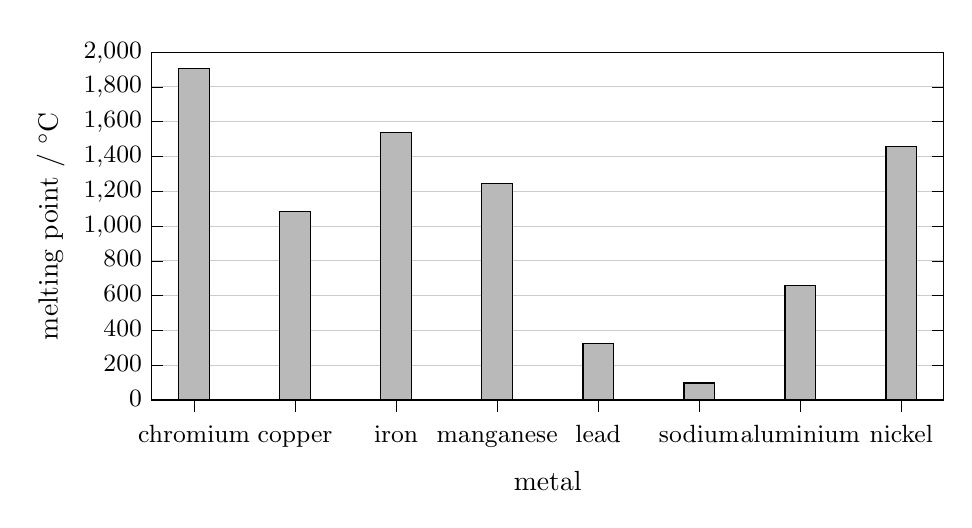
\begin{tikzpicture}
\begin{axis}[
  width=0.96\linewidth,
  height=60mm,
  ybar,
  bar width=11pt,
  ymin=0,
  ymax=2000,
  ylabel={melting point / $^{\circ}$C},
  xlabel={metal},
  symbolic x coords={chromium,copper,iron,manganese,lead,sodium,aluminium,nickel},
  xtick=data,
  typeset ticklabels with strut,
  ytick distance=200,
  ymajorgrids=true,
  grid style={gray!40},
  enlarge x limits=0.06,
  xtick pos=bottom,
  tick style={black},
  x tick label style={font=\small},
  y tick label style={font=\small}
]
\addplot[draw=black, fill=gray!55] coordinates {
  (chromium,1907)
  (copper,1084.62)
  (iron,1538)
  (lead,327.46)
  (manganese,1246)
  (sodium,97.79)
  (aluminium,660.32)
  (nickel,1455)
};
\end{axis}
\end{tikzpicture}
\end{center}
}
}

% Geschwindigkeitsverteilung bei drei Temperaturen
\newcommand{\TempChart}{
{
\begin{center}
	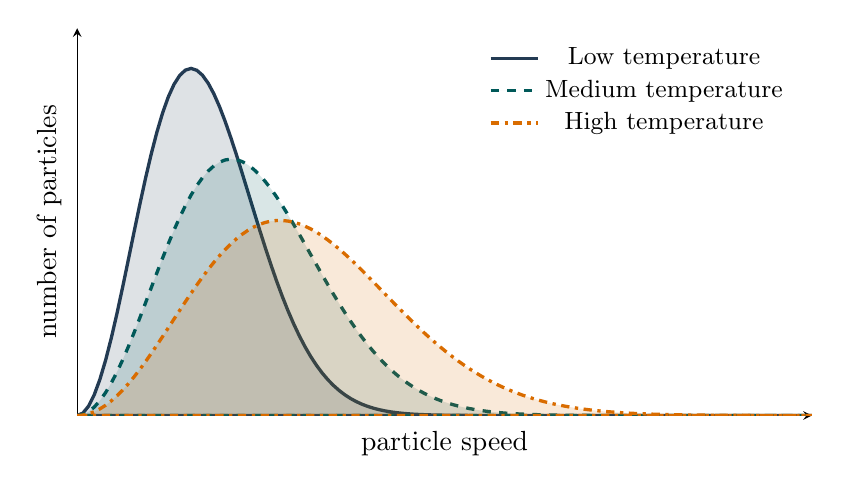
\begin{tikzpicture}
		\begin{axis}[
			width=0.90\linewidth,
			height=65mm,
			xmin=0, xmax=5,
			ymin=0, ymax=0.53,
			axis lines=left,
			xtick=\empty,
			ytick=\empty,
			xlabel={particle speed},
			ylabel={number of particles},
			legend style={
				draw=none,
				fill=none,
				font=\small,
				at={(0.98,0.98)},
				anchor=north east
			},
			samples=130,
			domain=0:5
			]
			
			% Niedrige Temperatur
			\addplot[
			very thick, DeepBlue,
			fill=DeepBlue, fill opacity=0.15
			] {x^2/(0.6^1.5)*exp(-x^2/0.6)} \closedcycle;
			\addlegendentry{Low temperature}
			
			% Mittlere Temperatur
			\addplot[
			very thick, dashed, teal!70!black,
			fill=teal!70!black, fill opacity=0.15
			] {x^2/(1.1^1.5)*exp(-x^2/1.1)} \closedcycle;
			\addlegendentry{Medium temperature}
			
			% Hohe Temperatur
			\addplot[
			very thick, dashdotted, orange!85!black,
			fill=orange!85!black, fill opacity=0.15
			] {x^2/(1.9^1.5)*exp(-x^2/1.9)} \closedcycle;
			\addlegendentry{High temperature}
			
		\end{axis}
	\end{tikzpicture}
\end{center}
}
}

% --- Teilchenbilder fuer homogeneous / heterogeneous mixtures ---

\newcommand{\WideMixtureSketch}[1]{%
	\begin{tikzpicture}[x=1mm,y=1mm]
		\draw[line width=.35mm] (0.25,0) rectangle ++(65,33.5);
		\foreach \j in {0,...,7}{%
			\foreach \i in {0,...,14}{%
				\pgfmathsetmacro{\xx}{3+4.15*\i+mod(\j,2)*1.5}
				\pgfmathsetmacro{\yy}{2.5+4.05*\j}
				\pgfmathtruncatemacro{\kind}{#1}
				\ifcase\kind
				\filldraw[fill=white,draw=black,line width=.2mm] (\xx,\yy) circle (1.8mm);
				\or
				\filldraw[fill=gray!60,draw=black,line width=.2mm] (\xx,\yy) circle (1.8mm);
				\else
				\filldraw[fill=black,draw=black,line width=.2mm] (\xx,\yy) circle (1.8mm);
				\fi
			}%
		}%
	\end{tikzpicture}%
}

% All three particle types are dispersed throughout the mixture.
\newcommand{\HomogeneousMixtureSketch}{%
	\WideMixtureSketch{mod(\i+14*\j,3)}%
}

% Three separate, liquid-like regions; no different densities or particle sizes.
\newcommand{\HeterogeneousMixtureSketch}{%
	\WideMixtureSketch{(\yy<11) ? 0 : ((\yy<19) ? 1 : 2)}%
}
% ============================================================
% Native LaTeX replacements for simple diagrams / worksheets.
% Original image files remain in images/ for reference.
% ============================================================

% Replaces images/scientific_cycle.png and images/brown_cycle.png.
% Unlabelled scientific cycle worksheet: keep the boxes empty.
\newcommand{\ScientificCycleFigure}{%
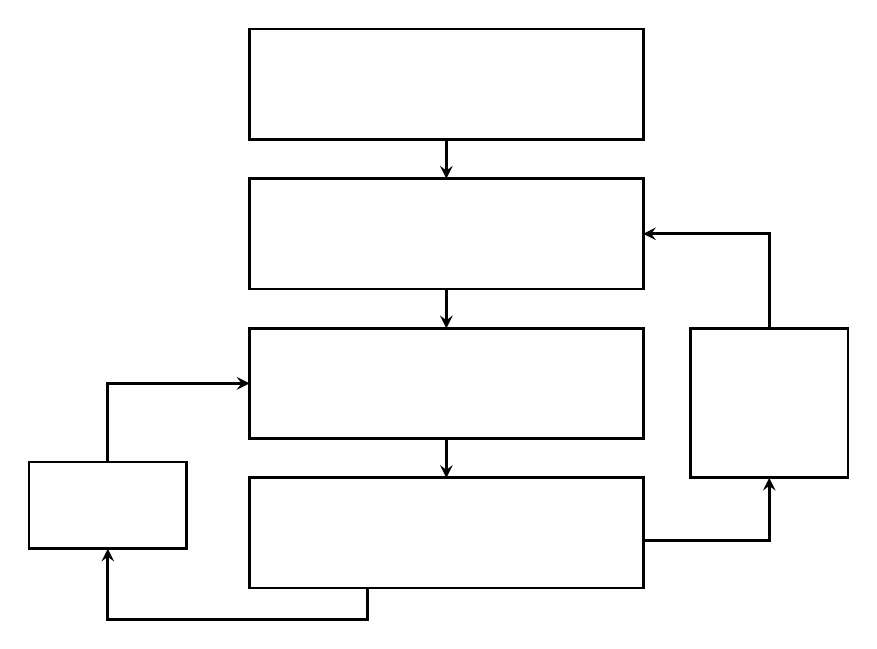
\begin{tikzpicture}[x=1mm,y=1mm,>=stealth,
  box/.style={draw=black,line width=.35mm,fill=white}]
  \draw[box] (-24,67) rectangle (26,81);
  \draw[box] (-24,48) rectangle (26,62);
  \draw[box] (-24,29) rectangle (26,43);
  \draw[box] (-24,10) rectangle (26,24);
  \draw[box] (-52,15) rectangle (-32,26);
  \draw[box] (32,24) rectangle (52,43);
  \draw[->,line width=.35mm] (1,67)--(1,62);
  \draw[->,line width=.35mm] (1,48)--(1,43);
  \draw[->,line width=.35mm] (1,29)--(1,24);
  % Loops from the result back to another step or question.
  \draw[->,line width=.35mm] (-9,10)--(-9,6)--(-42,6)--(-42,15);
  \draw[->,line width=.35mm] (-42,26)--(-42,36)--(-24,36);
  \draw[->,line width=.35mm] (26,16)--(42,16)--(42,24);
  \draw[->,line width=.35mm] (42,43)--(42,55)--(26,55);
\end{tikzpicture}%
}

% Replaces images/image13.png (blank 100 mL graduated cylinder).
\newcommand{\GraduatedCylinderFigure}{%
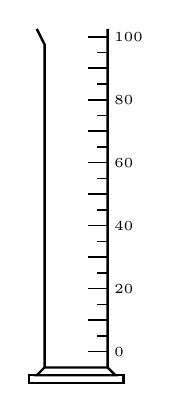
\begin{tikzpicture}[x=1mm,y=1mm,>=stealth]
  \draw[line width=.3mm] (1,47)--(2,45)--(2,4)--(10,4)--(10,47);
  \draw[line width=.3mm] (2,4)--(1,3)--(11,3)--(10,4);
  \draw[line width=.3mm] (0,2) rectangle (12,3);
  \foreach \i in {0,...,20}{%
    \pgfmathsetmacro{\yy}{6+\i*2}
    \draw[line width=.2mm] (10,\yy)--({ifthenelse(mod(\i,2)==0,7.5,8.6)},\yy);
  }
  \foreach \v/\yy in {0/6,20/14,40/22,60/30,80/38,100/46}{%
    \node[font=\tiny,anchor=west,inner sep=0.4mm] at (10.4,\yy) {\v};
  }
\end{tikzpicture}%
}

% Replaces images/image21.png: empty state-of-matter boxes and arrows.
\newcommand{\StateChangesWorksheetFigure}{%
	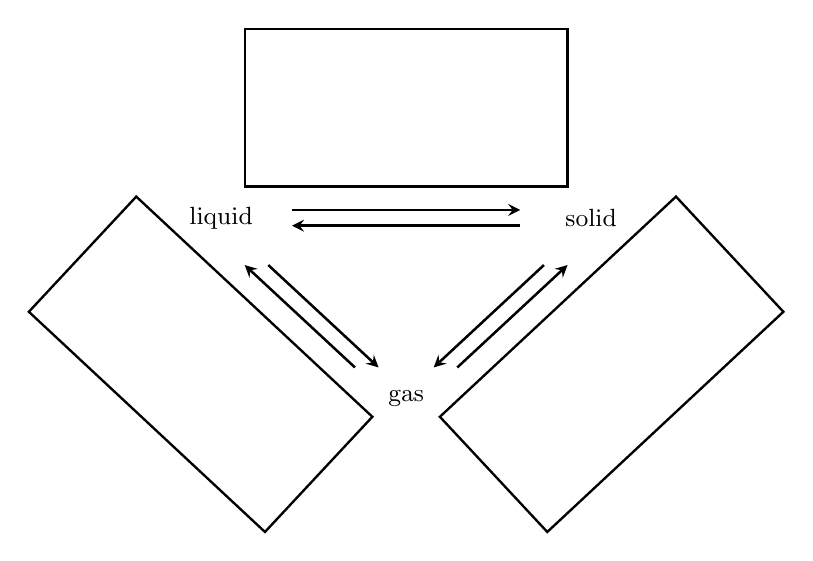
\begin{tikzpicture}[x=1mm,y=1mm,>=stealth,
		every node/.style={font=\small}]
		
		% Top rectangle
		\draw[line width=.3mm]
		(37,35) rectangle (78,55);
		
		% Left rectangle: parallel to liquid-gas arrows
		\begin{scope}[shift={(31.4,12.4)},rotate=-43]
			\draw[line width=.3mm]
			(-20.5,-10) rectangle (20.5,10);
		\end{scope}
		
		% Right rectangle: parallel to solid-gas arrows
		\begin{scope}[shift={(83.6,12.4)},rotate=43]
			\draw[line width=.3mm]
			(-20.5,-10) rectangle (20.5,10);
		\end{scope}
		
		% States of matter
		\node at (34,31) {liquid};
		\node at (81,31) {solid};
		\node at (57.5,8) {gas};
		
		% Liquid <-> Solid
		\draw[->,line width=.32mm] (43,32)--(72,32);
		\draw[->,line width=.32mm] (72,30)--(43,30);
		
		% Liquid <-> Gas
		\draw[->,line width=.32mm] (40,25)--(54,12);
		\draw[->,line width=.32mm] (51,12)--(37,25);
		
		% Solid <-> Gas
		\draw[->,line width=.32mm] (75,25)--(61,12);
		\draw[->,line width=.32mm] (64,12)--(78,25);
		
	\end{tikzpicture}%
}

% Replaces images/diffusion_diagram.png (two boxes and an arrow).
\newcommand{\DiffusionWorksheetFigure}{%
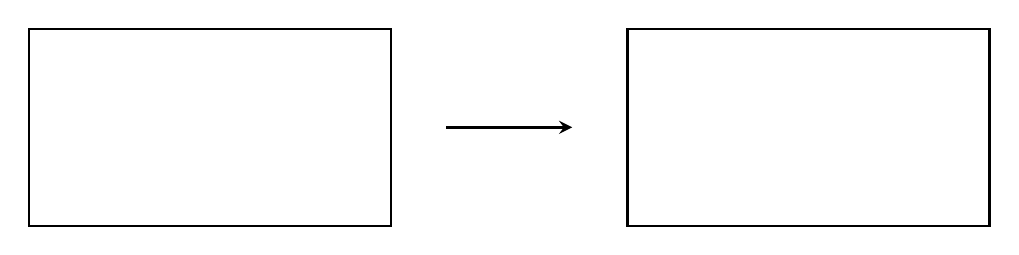
\begin{tikzpicture}[x=1mm,y=1mm,>=stealth]
  \draw[line width=.32mm] (0,0) rectangle (46,25);
  \draw[line width=.32mm] (76,0) rectangle (122,25);
  \draw[->,line width=.38mm] (53,12.5)--(69,12.5);
\end{tikzpicture}%
}

% Replaces images/mixtures_ex20.png (four labelled blank drawing spaces).
\newcommand{\MixtureDrawingWorksheetFigure}{%
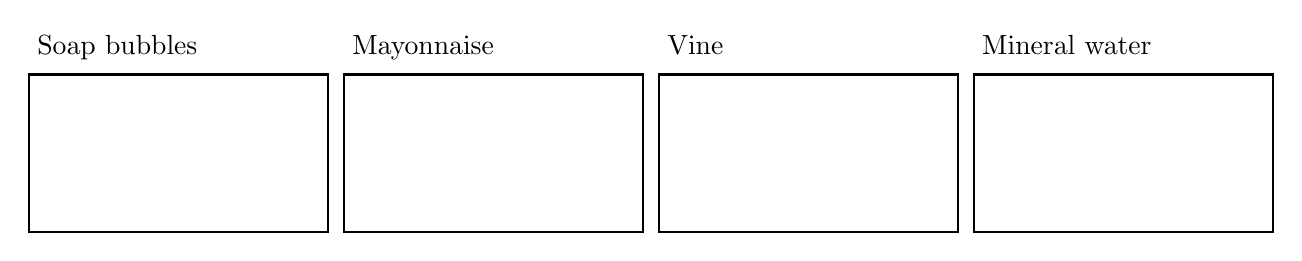
\begin{tikzpicture}[x=1mm,y=1mm]
  \foreach \n/\label in {0/Soap bubbles,1/Mayonnaise,2/Vine,3/Mineral water}{%
    \draw[line width=.32mm] ({40*\n},0) rectangle ({38+40*(\n)},20);
    \node[anchor=north west,inner sep=1mm]
      at ({40*\n},26) {\label};
  }
\end{tikzpicture}%
}

% Replaces images/image43.jpeg (pure substance / element / compound).
\newcommand{\PureSubstanceClassificationFigure}{%
	\resizebox{\linewidth}{!}{%
		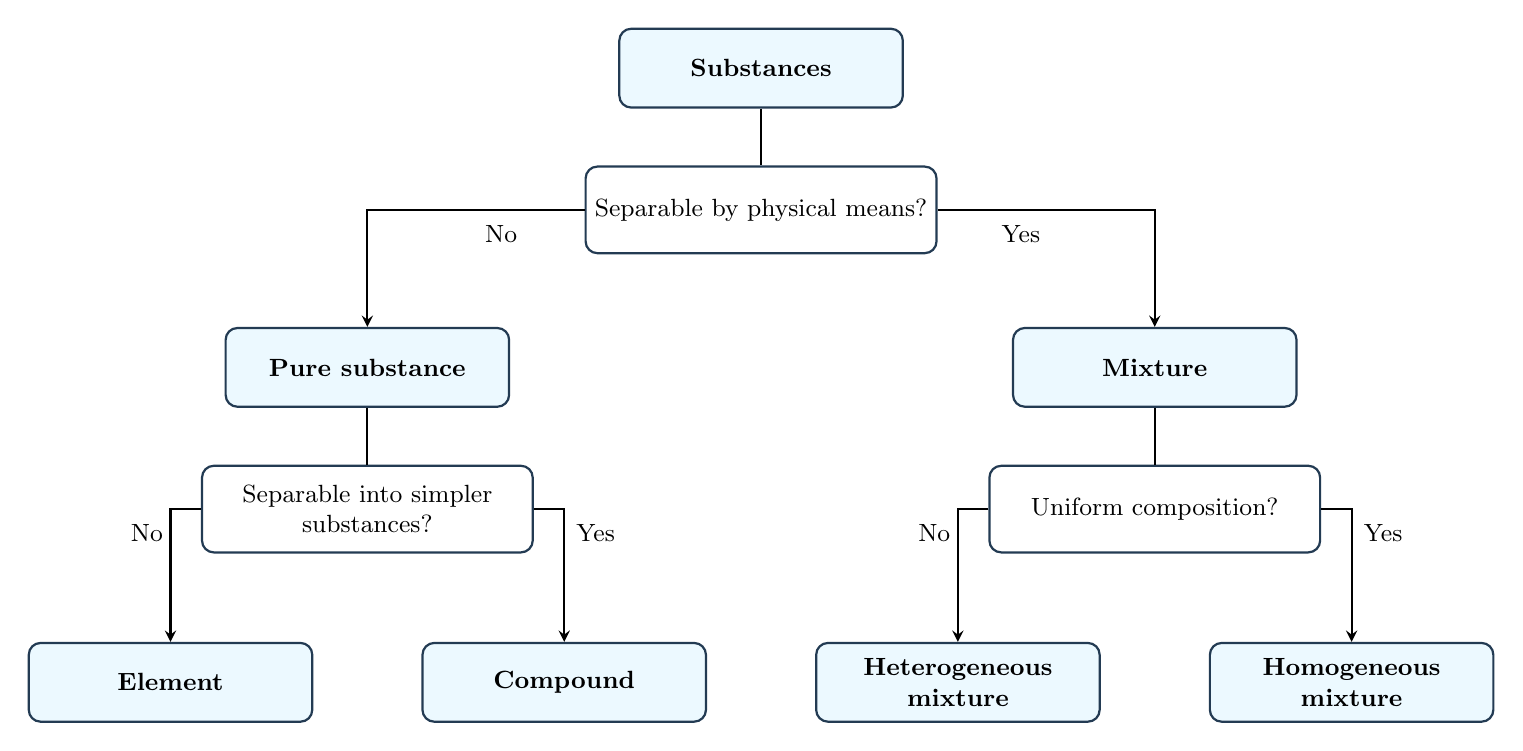
\begin{tikzpicture}[x=1mm,y=1mm,>=stealth,
			head/.style={
				draw=DeepBlue,
				rounded corners=1.5mm,
				thick,
				fill=InfoBlue,
				align=center,
				font=\bfseries\small,
				minimum width=36mm,
				minimum height=10mm
			},
			qbox/.style={
				draw=DeepBlue,
				rounded corners=1.5mm,
				thick,
				fill=white,
				align=center,
				font=\small,
				minimum width=42mm,
				minimum height=11mm
			}
			]
			
			% Top level
			\node[head] (sub) at (85,72) {Substances};
			
			% First decision
			\node[qbox] (phys) at (85,54)
			{Separable by physical means?};
			
			% Second level
			\node[head] (pure) at (35,34) {Pure substance};
			\node[head] (mix)  at (135,34) {Mixture};
			
			% Pure substance decision
			\node[qbox] (chem) at (35,16)
			{Separable into simpler\\substances?};
			
			% Mixture decision
			\node[qbox] (uniform) at (135,16)
			{Uniform composition?};
			
			% Final classes
			\node[head] (elem) at (10,-6) {Element};
			\node[head] (comp) at (60,-6) {Compound};
			\node[head] (hetero) at (110,-6) {Heterogeneous\\mixture};
			\node[head] (homo) at (160,-6) {Homogeneous\\mixture};
			
			% Connections top
			\draw[-,thick] (sub.south) -- (phys.north);
			
			\draw[->,thick] (phys.west) -- (35,54) -- (pure.north);
			\draw[->,thick] (phys.east) -- (135,54) -- (mix.north);
			
			\node[font=\small,fill=white,inner sep=1pt] at (52,51) {No};
			\node[font=\small,fill=white,inner sep=1pt] at (118,51) {Yes};
			
			% Pure branch
			\draw[-,thick] (pure.south) -- (chem.north);
			\draw[->,thick] (chem.west) -- (10,16) -- (elem.north);
			\draw[->,thick] (chem.east) -- (60,16) -- (comp.north);
			
			\node[font=\small,fill=white,inner sep=1pt] at (7,13) {No};
			\node[font=\small,fill=white,inner sep=1pt] at (64,13) {Yes};
			
			% Mixture branch
			\draw[-,thick] (mix.south) -- (uniform.north);
			\draw[->,thick] (uniform.west) -- (110,16) -- (hetero.north);
			\draw[->,thick] (uniform.east) -- (160,16) -- (homo.north);
			
			\node[font=\small,fill=white,inner sep=1pt] at (107,13) {No};
			\node[font=\small,fill=white,inner sep=1pt] at (164,13) {Yes};
			
		\end{tikzpicture}%
	}%
}

% Replaces images/physical_summary.png.
\newcommand{\PhysicalProcessSummaryFigure}{%
\begin{tikzpicture}[x=1mm,y=1mm,>=stealth]
  \foreach \x/\y in {2/5,9/13,21/19,8/23,26/8,18/4}{\draw[line width=.25mm] (\x,\y) rectangle ++(3.5,3.5);}
  \foreach \x/\y in {55/7,47/18,45/10,57/21}{\draw[line width=.25mm] (\x,\y)--++(4,0)--++(-2,4)--cycle;}
  \node at (36,14) {$+$};
  \draw[->,thick] (68,16)--(89,16);
  \draw[->,thick] (89,12)--(68,12);
  \foreach \x/\y in {101/19,109/11,102/4,124/0,133/20,136/11}{\draw[line width=.25mm] (\x,\y) rectangle ++(3.5,3.5);}
  \foreach \x/\y in {116/21,126/13,141/3,117/3}{\draw[line width=.25mm] (\x,\y)--++(4,0)--++(-2,4)--cycle;}
\end{tikzpicture}%
}

% Replaces images/chemical_summary.png: differently shaped new products.
\newcommand{\ChemicalReactionSummaryFigure}{%
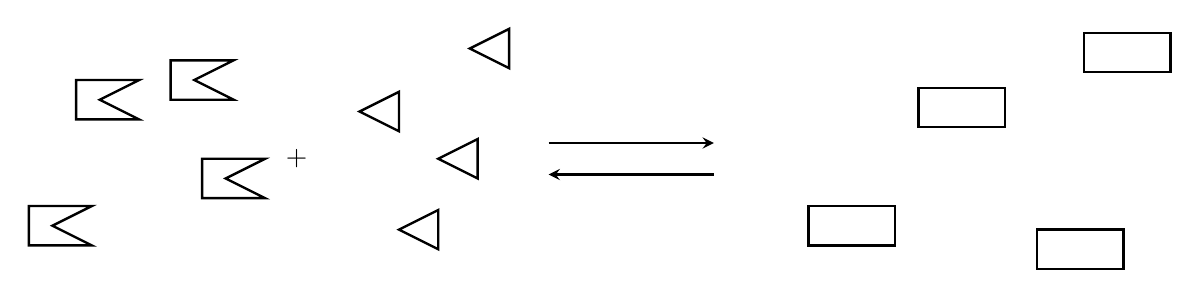
\begin{tikzpicture}[x=1mm,y=1mm,>=stealth]
  \foreach \x/\y in {2/3,8/19,24/9,20/21.5}{%
    \draw[line width=.3mm] (\x,\y)--++(8,0)--++(-5,2.5)--++(5,2.5)--++(-8,0)--cycle;
  }
  \foreach \x/\y in {49/5,44/20,58/28,54/14}{\draw[line width=.3mm] (\x,\y)--++(5,-2.5)--++(0,5)--cycle;}
  \node at (36,14) {$+$};
  \draw[->,thick] (68,16)--(89,16);
  \draw[->,thick] (89,12)--(68,12);
  \foreach \x/\y in {101/3,115/18,136/25,130/0}{\draw[line width=.3mm] (\x,\y) rectangle ++(11,5);}
\end{tikzpicture}%
}

% Replaces images/filtration_diagram.png (submicroscopic / macroscopic).
\newcommand{\FiltrationFigure}{%
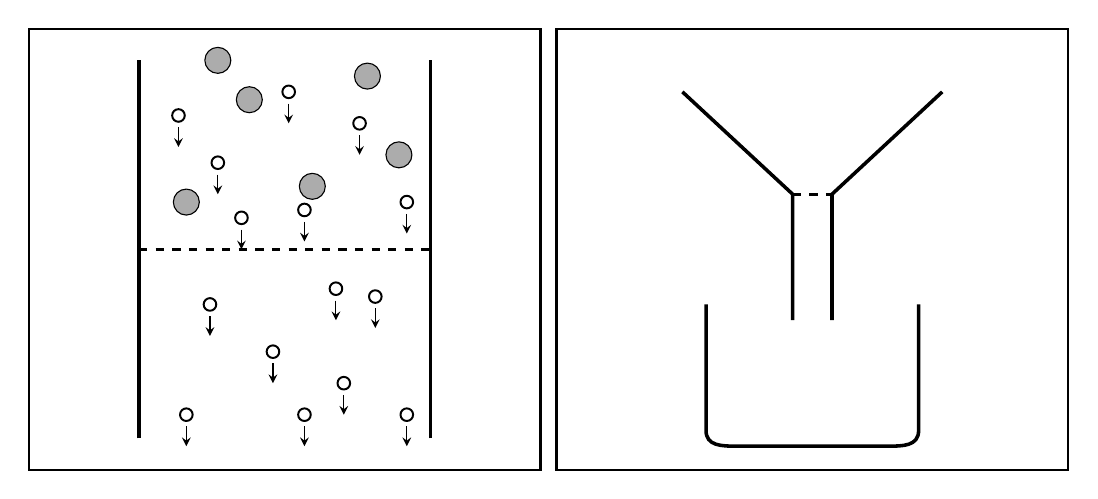
\begin{tikzpicture}[x=1mm,y=1mm,>=stealth]
  \draw[line width=.3mm] (0,0) rectangle (65,56);
  \draw[line width=.3mm] (67,0) rectangle (132,56);
  % Particle-level filtering: solvent through filter, larger solid particles above.
  \draw[line width=.45mm] (14,4)--(14,52) (51,4)--(51,52);
  \draw[very thick,dashed] (14,28)--(51,28);
  \foreach \x/\y in {20/34,28/47,36/36,43/50,47/40,24/52}{%
    \filldraw[fill=gray!65,draw=black] (\x,\y) circle (1.65mm);
  }
  \foreach \x/\y in {19/45,24/39,33/48,42/44,48/34,23/21,31/15,39/23,40/11,20/7,48/7,35/7,27/32,35/33,44/22}{%
    \draw[line width=.25mm,fill=white] (\x,\y) circle (0.8mm);
    \draw[->,thin] (\x,\y-1.5)--(\x,\y-4);
  }
  % Macroscopic set-up: funnel, stem and collecting beaker.
  \draw[line width=.45mm] (83,48)--(97,35)--(97,19);
  \draw[line width=.45mm] (116,48)--(102,35)--(102,19);
  \draw[very thick,dashed] (97,35)--(102,35);
  \draw[line width=.45mm] (86,21)--(86,5) .. controls (86,3) and (88,3) .. (90,3)--(109,3) .. controls (111,3) and (113,3) .. (113,5)--(113,21);
\end{tikzpicture}%
}

% Replaces images/image20.jpg (gas bubbles in a liquid).
% Grey = liquid, closely packed but slightly irregular; white = gas, far apart.
\newcommand{\GasBubblesInLiquidFigure}{%
	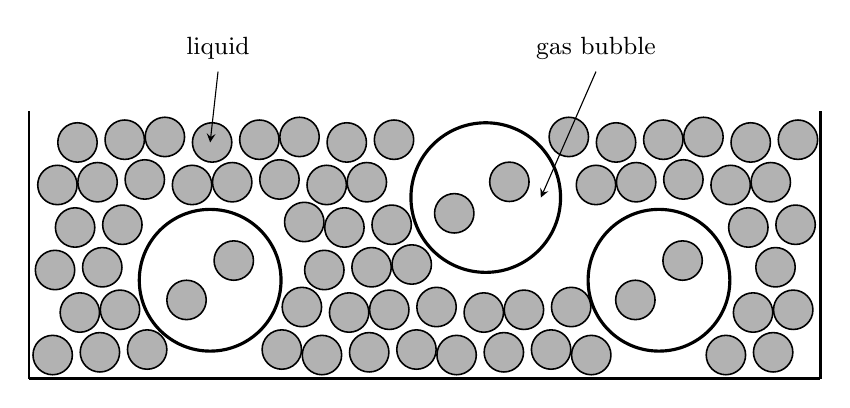
\begin{tikzpicture}[x=1mm,y=1mm,>=stealth]
		\draw[line width=.35mm] (0,0)--(0,34) (100.5,0)--(100.5,34) (0,0)--(100.5,0);
		% Use the *actual* centres/radii of the bubbles when leaving liquid out.
		\foreach \j in {0,...,5}{%
			\foreach \i in {0,...,16}{%
				\pgfmathsetmacro{\px}{3+5.7*\i+2.85*mod(\j,2)+0.30*mod(7*\i+11*\j,3)}
				\pgfmathsetmacro{\py}{3+5.4*\j+0.35*mod(13*\i+3*\j,3)}
				% Add the liquid-particle radius as a safety margin.
				\pgfmathtruncatemacro{\blocked}{%
					((\px-23)^2+(\py-12.5)^2<11.5^2) ||
					((\px-58)^2+(\py-23)^2<12^2) ||
					((\px-80)^2+(\py-12.5)^2<11.5^2)}
				\ifnum\blocked=0
				\filldraw[fill=gray!60,draw=black,line width=.2mm] (\px,\py) circle (2.5mm);
				\fi
			}%
		}%
		\draw[line width=.4mm] (23,12.5) circle[radius=9mm];
		\draw[line width=.4mm] (58,23) circle[radius=9.5mm];
		\draw[line width=.4mm] (80,12.5) circle[radius=9mm];
		\foreach \x/\y in {20/10,26/15,54/21,61/25,77/10,83/15}{%
			\filldraw[fill=gray!60,draw=black,line width=.2mm] (\x,\y) circle (2.5mm);
		}%
		\node[font=\small] at (24,42) {liquid};
		\node[font=\small] at (72,42) {gas bubble};
		\draw[->] (24,39)--(23,30);
		\draw[->] (72,39)--(65,23);
	\end{tikzpicture}%
}

% Replaces images/image16.jpeg (Brownian motion due to random collisions).
\newcommand{\BrownianCollisionFigure}{%
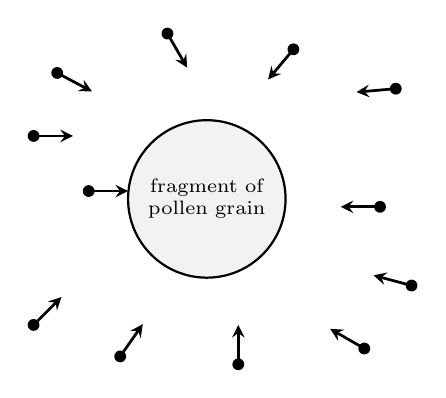
\begin{tikzpicture}[x=1mm,y=1mm,>=stealth]
  \draw[thick,fill=gray!10] (26,24) circle (10mm);
  \node[font=\scriptsize,align=center,text width=17mm]
      at (26,24) {fragment of\\pollen grain};
  \foreach \x/\y/\a in
    {4/8/45,11/25/0,7/40/-28,21/45/-60,37/43/-130,
      50/38/185,48/23/180,46/5/150,30/3/90,15/4/55,
      4/32/0,52/13/165}{%
    \fill (\x,\y) circle (0.75mm);
    \draw[->,line width=.35mm] (\x,\y)--++(\a:5mm);
  }
\end{tikzpicture}%
}

% Replaces images/image17.jpeg (surface reaction of two solids).
% White A-particles and grey B-particles; black C-particles are the products.
\newcommand{\SolidSurfaceReactionFigure}{%
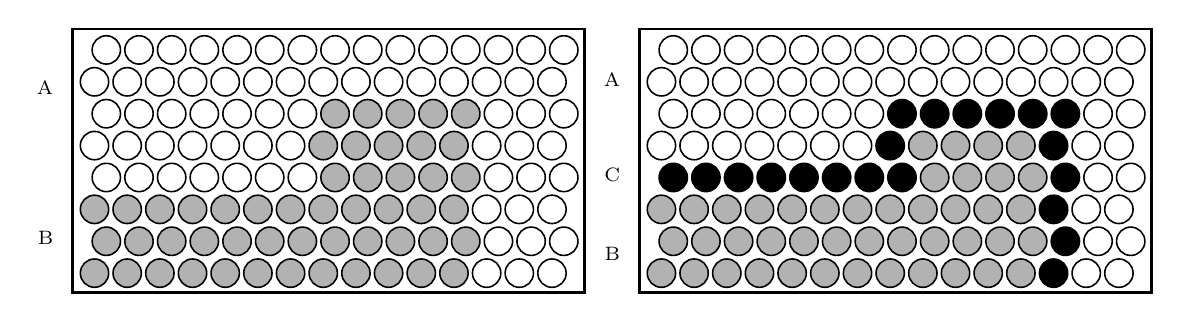
\begin{tikzpicture}[x=1mm,y=1mm,>=stealth]
  \foreach \p in {0,1}{%
    \pgfmathsetmacro{\xshift}{72*\p}
    \draw[line width=.35mm] (\xshift+0.25,0) rectangle ++(65,33.5);
    \foreach \j in {0,...,7}{%
      \foreach \i in {0,...,14}{%
        \pgfmathsetmacro{\xx}{\xshift+3+4.15*\i+mod(\j,2)*1.5}
        \pgfmathsetmacro{\yy}{2.5+4.05*\j}
        \pgfmathtruncatemacro{\isB}{(\i<8 && \j<3) || (\i>6 && \j<6 && \i<12)}
        \pgfmathtruncatemacro{\isC}{\p==1 && ((\i<=7 && \j==3) || (\i==12 && \j<=5) || (\i==7 && \j>=4 && \j<=5) || (\i>=7 && \i<=12 && \j== 5))}
        \ifnum\isC=1
          \filldraw[fill=black,draw=black,line width=.2mm] (\xx,\yy) circle (1.8mm);
        \else
          \ifnum\isB=1
            \filldraw[fill=gray!60,draw=black,line width=.2mm] (\xx,\yy) circle (1.8mm);
          \else
            \filldraw[fill=white,draw=black,line width=.2mm] (\xx,\yy) circle (1.8mm);
          \fi
        \fi
      }
    }
  }
  \node[font=\scriptsize,anchor=east] at (-1,26) {A};
  \node[font=\scriptsize,anchor=east] at (-1,7) {B};
  \node[font=\scriptsize,anchor=east] at (71,27) {A};
  \node[font=\scriptsize,anchor=east] at (71,15) {C};
  \node[font=\scriptsize,anchor=east] at (71,5) {B};
\end{tikzpicture}%
}

% Three car models
% Original image: images/three-car-models.png

\newcommand{\CarModelPanel}[2]{%
	\begin{minipage}[c]{0.314\linewidth}
		\centering
		\fbox{%
			\begin{minipage}[c][33mm][c]{%
					\dimexpr\linewidth-2\fboxsep-2\fboxrule\relax}
				\centering
				\includegraphics[
				width=\linewidth,
				height=31mm,
				keepaspectratio,
				trim={#1bp 11bp #2bp 11bp},
				clip
				]{images/three-car-models.png}
			\end{minipage}%
		}%
	\end{minipage}%
}

\newcommand{\CarModelsFigure}{%
	\begin{center}
		\CarModelPanel{12}{602}\hfill
		\CarModelPanel{294}{328}\hfill
		\CarModelPanel{567}{15}
	\end{center}%
}

% Solubility Curves
% Replaces images/image22.png
% Data points approximated from the original figure.

\newcommand{\SolubilityCurvesFigure}{%
	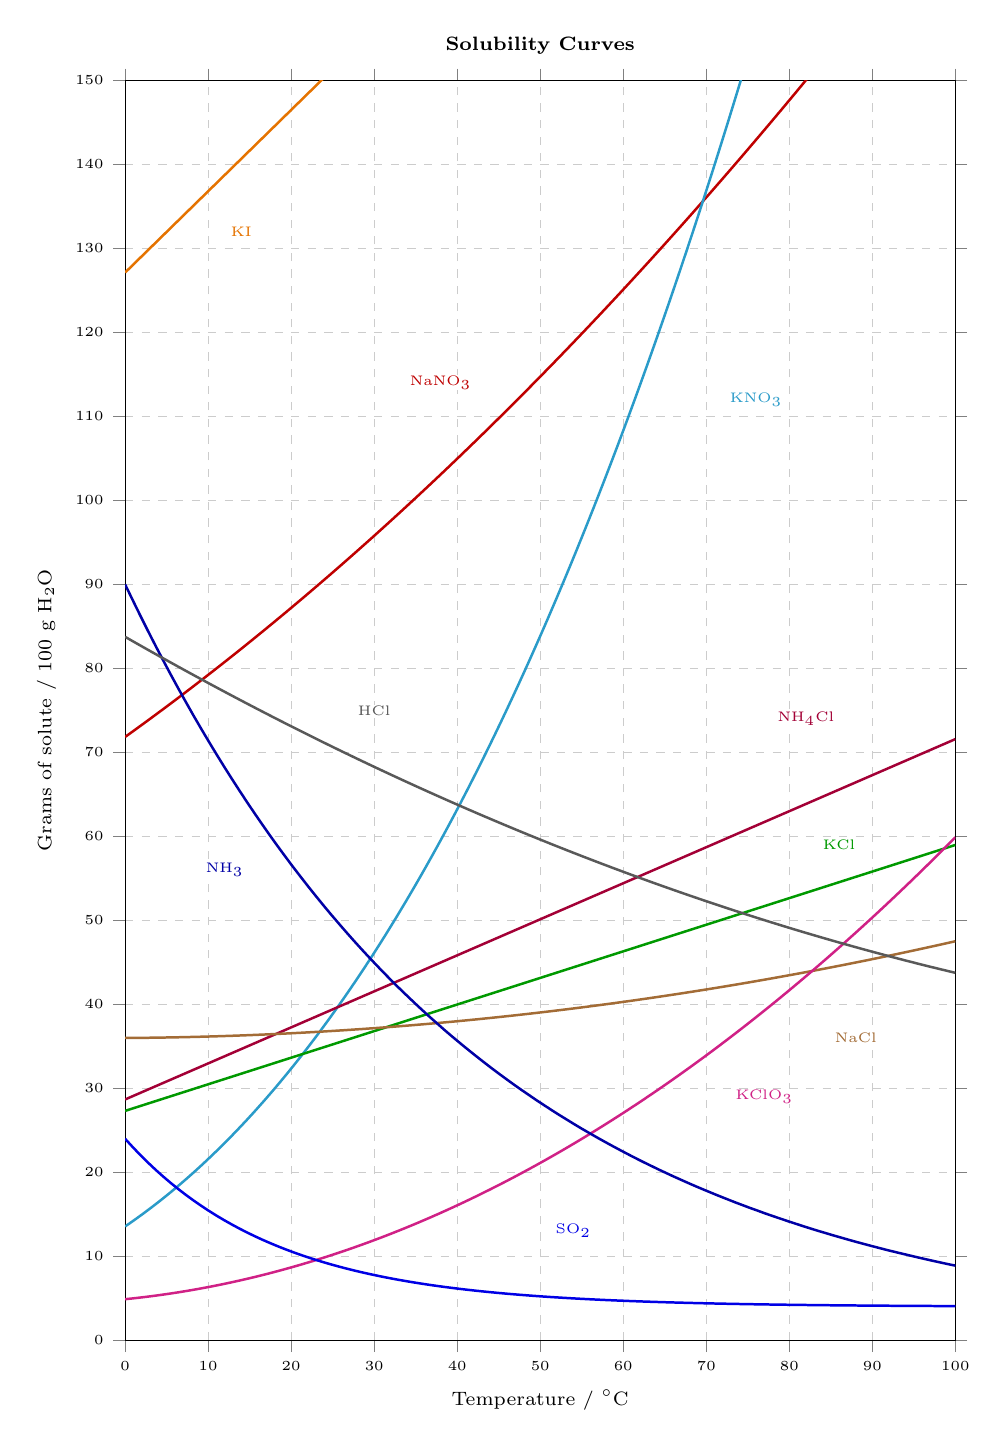
\begin{tikzpicture}
		\begin{axis}[
			width=\linewidth,
			height=1.45\linewidth,
			title={Solubility Curves},
			title style={font=\scriptsize\bfseries},
			xmin=0, xmax=100,
			ymin=0, ymax=150,
			xtick={0,10,...,100},
			ytick={0,10,...,150},
			xmajorgrids=true,
			ymajorgrids=true,
			grid style={gray!40,dashed},
			axis lines=box,
			tick align=outside,
			tick label style={font=\tiny},
			label style={font=\scriptsize},
			xlabel={Temperature / $^\circ$C},
			ylabel={Grams of solute / 100 g H$_2$O},
			every axis plot/.append style={
				mark=none,
				line width=0.9pt,
				samples=110
			},
			clip=true
			]
			
			% Potassium iodide (KI)
			\addplot[orange!90!black, domain=0:26]
			{127.13 + x*(0.96808)};
			
			% Sodium nitrate (NaNO3)
			\addplot[red!75!black, domain=0:84]
			{71.84 + x*(0.70881 + 0.002984*x)};
			
			% Potassium nitrate (KNO3)
			\addplot[cyan!80!black, domain=0:76]
			{13.56 + x*(0.67378 + x*(0.012395 + 0.00004494*x))};
			
			% Ammonium chloride (NH4Cl)
			\addplot[purple!85!black, domain=0:100]
			{28.68 + x*(0.42902)};
			
			% Potassium chloride (KCl)
			\addplot[green!60!black, domain=0:100]
			{27.32 + x*(0.31661)};
			
			% Sodium chloride (NaCl)
			\addplot[brown!85!black, domain=0:100]
			{36 + x*(0.00636 + x*(0.001088))};
			
			% Potassium chlorate (KClO3)
			\addplot[magenta!85!black, domain=0:100]
			{4.90 + x*(0.09895 + 0.0045105*x)};
			
			% Ammonia (NH3)
			\addplot[blue!65!black, domain=0:100]
			{90*exp(-0.02314*x)};
			
			% Hydrogen chloride (HCl)
			\addplot[gray!70!black, domain=0:100]
			{83.76 + x*(-0.5655 + 0.001655*x)};
			
			% Sulphur dioxide (SO2)
			\addplot[blue!90!black, domain=0:100]
			{4 + 20*exp(-x/18)};
			
			% Labels inside the graph
			\node[font=\tiny,text=orange!90!black,fill=white,
			inner sep=0.3pt] at (axis cs:14,132) {KI};
			
			\node[font=\tiny,text=red!75!black,fill=white,
			inner sep=0.3pt] at (axis cs:38,114) {NaNO$_3$};
			
			\node[font=\tiny,text=cyan!80!black,fill=white,
			inner sep=0.3pt] at (axis cs:76,112) {KNO$_3$};
			
			\node[font=\tiny,text=purple!85!black,fill=white,
			inner sep=0.3pt] at (axis cs:82,74) {NH$_4$Cl};
			
			\node[font=\tiny,text=green!60!black,fill=white,
			inner sep=0.3pt] at (axis cs:86,59) {KCl};
			
			\node[font=\tiny,text=brown!85!black,fill=white,
			inner sep=0.3pt] at (axis cs:88,36) {NaCl};
			
			\node[font=\tiny,text=magenta!85!black,fill=white,
			inner sep=0.3pt] at (axis cs:77,29) {KClO$_3$};
			
			\node[font=\tiny,text=blue!65!black,fill=white,
			inner sep=0.3pt] at (axis cs:12,56) {NH$_3$};
			
			\node[font=\tiny,text=gray!70!black,fill=white,
			inner sep=0.3pt] at (axis cs:30,75) {HCl};
			
			\node[font=\tiny,text=blue!90!black,fill=white,
			inner sep=0.3pt] at (axis cs:54,13) {SO$_2$};
			
		\end{axis}
	\end{tikzpicture}%
}

% ------------------------------------------------------------
% Particle-model mixture types for Exercise 1-27.
% Two particle types ONLY, as requested. The state is shown by spacing:
% solid = regular close packing; liquid = disordered close packing;
% gas = widely spaced particles. Same grey/white palette as above.
% ------------------------------------------------------------
\tikzset{
	mixA/.style={draw=black, fill=white},
	mixB/.style={draw=black, fill=gray!60}
}

\newcommand{\MixtureBox}[1]{%
	\begin{tikzpicture}[x=1mm,y=1mm]
		\draw[thick] (0,0) rectangle (38,28);
		#1
	\end{tikzpicture}%
}

% 1) Solid aerosol: compact ordered solid fragments dispersed in a gas.
\newcommand{\SolidAerosolFigure}{%
	\MixtureBox{%
		% Widely separated gas particles (A).
		\foreach \x/\y in {
			4/24,11/24,19/25,32/24,35/17,4/17,
			18/16,31/13,4/9,21/7,30/5,19/21}{%
			\filldraw[mixA] (\x,\y) circle[radius=1.35mm];
		}%
		% Two ordered solid clusters (B), both on the same lattice spacing.
		\foreach \x/\y in {
			8/4.75,12.15/4.75,16.3/4.75,8/8.8,12.15/8.8,16.3/8.8,
			24/16.7,28.15/16.7,24/20.75,28.15/20.75}{%
			\filldraw[mixB] (\x,\y) circle[radius=1.8mm];
		}%
	}%
}

% 2) Liquid aerosol: irregular, close-packed liquid droplets in a gas.
\newcommand{\LiquidAerosolFigure}{%
	\MixtureBox{%
		\foreach \x/\y in {
			4/23,21/24,30/23,35/21,4/13,19/11,
			35/14,5/5,16/5,21/16,35/5}{%
			\filldraw[mixA] (\x,\y) circle[radius=1.35mm];
		}%
		\foreach \x/\y in {
			10/19.5,13.8/20,9.3/15.8,13.1/16.2,16.8/18,
			25.2/10.6,29/11,24.7/6.8,28.5/7.2,32/9}{%
			\filldraw[mixB] (\x,\y) circle[radius=1.75mm];
		}%
	}%
}

% 3) Alloy: different atoms on an ordered, closely packed solid lattice.
\newcommand{\AlloyFigure}{%
	\MixtureBox{%
		\foreach \j in {0,...,5}{%
			\foreach \i in {0,...,7}{%
				\pgfmathsetmacro{\xx}{4+4.1*\i+1.45*mod(\j,2)}
				\pgfmathsetmacro{\yy}{4+4.0*\j}
				\pgfmathtruncatemacro{\solute}{mod(3*\i+2*\j,7)<2}
				\ifnum\solute=1
				\filldraw[mixB] (\xx,\yy) circle[radius=1.8mm];
				\else
				\filldraw[mixA] (\xx,\yy) circle[radius=1.8mm];
				\fi
			}%
		}%
	}%
}

% Helper for both liquid solutions: same disordered, dense positions.
% Argument is the expression selecting the darker particle type.
\newcommand{\LiquidSolutionModel}[1]{%
	\MixtureBox{%
		\foreach \j in {0,...,5}{%
			\foreach \i in {0,...,7}{%
				\pgfmathsetmacro{\xx}{4.3+4.1*\i+1.25*mod(\j,2)+0.19*mod(7*\i+11*\j,5)}
				\pgfmathsetmacro{\yy}{3.2+4.05*\j+0.20*mod(13*\i+3*\j,5)}
				\pgfmathtruncatemacro{\solute}{#1}
				\ifnum\solute=1
				\filldraw[mixB] (\xx,\yy) circle[radius=1.62mm];
				\else
				\filldraw[mixA] (\xx,\yy) circle[radius=1.62mm];
				\fi
			}%
		}%
	}%
}

% 4) Homogeneous liquid mixture: comparable amounts of both components.
\newcommand{\LiquidSolutionFigureA}{%
	\LiquidSolutionModel{mod(3*\i+5*\j,7)<3}%
}

% 5) Gas mixture: separate, far-apart particles of both species.
\newcommand{\GasMixtureFigure}{%
	\MixtureBox{%
		\foreach \x/\y in {
			4/23,16/24,29/23,9/17,23/16,34/15,5/7,19/6,32/5}{%
			\filldraw[mixA] (\x,\y) circle[radius=1.35mm];
		}%
		\foreach \x/\y in {
			9/24,23/22,35/24,4/15,16/14,30/12,12/6,26/7}{%
			\filldraw[mixB] (\x,\y) circle[radius=1.35mm];
		}%
	}%
}

% 6) A second homogeneous liquid solution, with less of component B.
\newcommand{\LiquidSolutionFigureB}{%
	\LiquidSolutionModel{mod(5*\i+3*\j,11)<2}%
}

% Consistent 2 x 3 layout for Exercise 1-27.
\newcommand{\MixtureExampleCell}[1]{%
	\begin{minipage}[t]{0.31\linewidth}
		\centering
		#1\\[1mm]
	\end{minipage}%
}

\newcommand{\ExerciseOneTwentySevenMixturesFigure}{%
	\begin{center}
		\MixtureExampleCell{\SolidAerosolFigure}\hfill
		\MixtureExampleCell{\LiquidAerosolFigure}\hfill
		\MixtureExampleCell{\AlloyFigure}
		
		\vspace{4ex}
		
		\MixtureExampleCell{\LiquidSolutionFigureA}\hfill
		\MixtureExampleCell{\GasMixtureFigure}\hfill
		\MixtureExampleCell{\LiquidSolutionFigureB}
		
		\vspace{4ex}
		
	\end{center}%
}

\begin{document}
\pagenumbering{gobble}
% Source: 01 Properties_of_Matter 26(1).docx; formatting in layout.tex.
\OutlinedChapterTitle{\ScriptTitle}


\textbf{The students\ldots{}}


\Objective{know the definition of the term \textit{chemistry.}}

\Objective{know the GHS pictograms and their meanings.}

\Objective{understand why experiments are essential in science.}

\Objective{know the basic building blocks of a lab report and know how to write a lab report for an experiment.}

\Objective{\textbf{ know the definition of the particle model and are able to apply it to different situations.}}

\Objective{\textbf{ know what a chemical reaction is, can classify reactions as exothermic or endothermic and can draw the corresponding energy diagrams.}}

\Objective{can formulate reaction equations using names of substances and understand the process on a particle level.}

\Objective{know the definition of the term \textit{substance}}

\Objective{can convert from decimal to scientific to prefix notation and vice versa}

\Objective{can convert units}

\Objective{understand the material properties \textit{melting point }and \textit{boiling point} and know how different factors influence them.}

\Objective{know the characteristics of the states of matter and the transitions between them on the macroscopic level (= our daily lives) and on a particle level.}

\Objective{\textbf{understand the property }\textbf{\textit{solubility}}\textbf{ and know the different terms connected with solubility (solute, solvent, dissolved, saturated solution, solubility).}}

\Objective{understand solubility diagrams and can extract information of a diagram.}

\Objective{understand the material property \textit{density} and know how different factors influence it.}

\Objective{are able to solve simple problems concerning density.}

\Objective{understand the concept which explains the temperature of a substance.}

\Objective{know the term \textit{diffusion} and \textit{osmosis }and can explain them by using examples.}

\Objective{\textbf{ know and understand the terms }\textbf{\textit{homogeneous mixtures}}\textbf{ and }\textbf{\textit{heterogeneous mixtures}}\textbf{.}}

\Objective{know the names of the different types of mixtures and can draw them on a particle level and can name an example.}

\Objective{can name and describe a number of important separation methods.}

\Objective{understand the principles which lie behind these separation methods also on a particle level.}

\Objective{\textbf{ can use the terms }\textbf{\textit{pure substance}}\textbf{, }\textbf{\textit{mixture}}\textbf{, }\textbf{\textit{element}}\textbf{, and }\textbf{\textit{compound }}\textbf{to explain the division of matter which is commonly used in chemistry. }}

\Objective{understand all exercises and experiments}

\ObjectivesNote{Objectives in bold are also relevant for future exams}

\clearpage
\pagenumbering{arabic}
% Source: 01 Properties_of_Matter 26(1).docx; formatting in layout.tex.
% Bewaehrte Einleitungsseite aus der abgestimmten Layoutprobe.
% Druckseite 1 – Titelhierarchie, Infobox, Textumfluss und Vergleichstabelle.
\HOne{Introduction}
\HTwo{What Chemistry Is All About}
Have you ever wondered why ice melts and water evaporates? Why do leaves change colour in autumn? How does a battery produce electricity, or why does food last longer in a refrigerator?

Chemistry helps us answer these questions. It connects everyday observations with explanations about substances, their properties, and the changes they undergo. Chemistry helps explain why a match burns, how medicines are developed, and what happens inside distant stars.

\begin{InfoBox}
\BoxHeading{Definition of Chemistry}
\textbf{Chemistry} is the study of substances, their properties, and the changes they undergo.
\end{InfoBox}

\HThree{From practical knowledge to modern chemistry}
\HFour{Early practical chemistry}
Long before chemistry became a science, people extracted metals, fired clay to make ceramics and glass, and produced dyes. They knew \textit{how} to carry out these processes, but they could not yet explain \textit{why} they worked.

% Die antike Rezeptillustration ist ein freigestelltes Originalbild aus Word.
\begin{wrapfigure}[16]{r}{229.1pt}
 \vspace{-10pt}
 \includegraphics[width=229.1pt]{images/alchemy.jpeg}
\end{wrapfigure}
\HFour{Alchemy}
From antiquity onwards, alchemical traditions developed across many cultures, including ancient Egypt, China, India, the medieval Islamic civilisation, and Europe. Many alchemists tried to turn inexpensive metals into gold or silver. They did not succeed, but they developed useful techniques for heating, mixing, dissolving, and separating substances.

\HFour{The beginnings of modern chemistry}
In the seventeenth century, chemists increasingly focused on experiments and clearly defined substances. In 1661, \textbf{Robert Boyle} published \textit{The Sceptical Chymist}. He challenged the ancient idea that all matter consisted of earth, air, fire, and water and helped shape the modern concept of chemical elements.

\WFclear

As we study chemistry, we constantly move between two different levels:

\CompareBox
  {Macroscopic level}
  {What we can observe and measure directly, for example colour changes, temperature\ changes, or the formation of a gas.}
  {Submicroscopic level}
  {Models that explain observations using particles such as atoms, molecules, and ions, which are too small to see directly.}

\newpage
\HTwo{Chemistry Today}

Chemistry connects physics and biology. For a first overview, it is often described through four broad academic fields. In practice, these fields overlap and work together.


\par\smallskip

% Die vier akademischen Fachgebiete
\begin{description}[
  style=nextline,
  font=\bfseries\color{DeepBlue},
  leftmargin=0pt,
  labelsep=0pt,
  itemsep=1ex,
  parsep=0pt
]

\item[Physical chemistry]
Explains how and why chemical processes occur. It uses
ideas such as energy, temperature, pressure, and
reaction rate.

\textit{Example: Why does a reaction become faster
when the temperature rises?}

\item[Inorganic chemistry]
Studies elements and compounds that are not primarily
based on carbon, including metals, salts, minerals,
acids, bases, and crystals.

\textit{Example: How do metals react with acids?}

\item[Analytical chemistry]
Determines what a sample contains and how much of each
substance is present. It uses methods such as
chromatography.

\textit{Example: How much vitamin C is present
in a drink?}

\item[Organic chemistry]
Studies carbon-based compounds, including fuels,
plastics, medicines, sugars, fats, and many substances
found in living organisms.

\textit{Example: How can a medicine be synthesised?}

\end{description}

\par\smallskip


\HThree{Chemistry in research, industry and society}

Outside the traditional academic fields, chemists often work in interdisciplinary areas. These fields combine chemistry with medicine, biology, environmental science, technology, and industrial production. They can lead to careers in the pharmaceutical, energy, materials, environmental, and manufacturing industries. Here are a few examples:


\par\smallskip

% Interdisziplinaere Fachgebiete in zwei Spalten
\begin{tblr}{
  width=\linewidth,
  colspec={X[l,t] X[l,t]},
  colsep=8pt, rowsep=3pt,
  column{1}={leftsep=0pt},
  column{2}={rightsep=0pt}
}

\textbf{Biochemistry:}
chemical processes in living organisms
&
\textbf{Medicinal chemistry:}
discovery and development of medicines \\

\textbf{Neurochemistry:}
chemical processes in the nervous system and brain
&
\textbf{Environmental chemistry:}
chemical processes in nature and the effects of pollution \\

\textbf{Materials science:}
development and testing of new materials
&
\textbf{Nuclear chemistry:}
radioactive substances and nuclear processes \\

\textbf{Chemical engineering:}
safe and efficient large-scale chemical production
&
\textbf{Computational chemistry:}
computer models and simulations of molecules and reactions

\end{tblr}

\par\smallskip


\Exercise{Which area of chemistry sounds most interesting to you? Optional challenge: Find a real-world profession that uses this branch of chemistry.}

\newpage
\HTwo{GHS Hazard Pictograms}

In 2008 the EU decided to adopt the Globally Harmonized System of Classification and Labelling of Chemicals, GHS system for short. It was designed to replace the various classification and labelling standards used in different countries by using consistent criteria for classification and labelling on a world-wide level.


The table on the following page shows the GHS pictograms together with their meaning and examples. Complete the table by describing the main hazard represented by each pictogram.


{\small

\begin{StandardTable}{
  colspec={X[0.85,c,m] X[1.1,c,m] X[1.25,c,m]},
  row{2-10}={ht=17mm}
}

{GHS pictogram} & {description of danger} & {example} \\ 

\raisebox{-0.45\height}{\includegraphics[height=14mm]{images/image3.png}} & {} & {Botulinum toxin (Botox)} \\ 

\raisebox{-0.45\height}{\includegraphics[height=14mm]{images/image4.png}} & {} & {petrol \textsuperscript{\textit{BE}}} \\ 

\raisebox{-0.45\height}{\includegraphics[height=14mm]{images/image5.png}} & {} & {potassium nitrate\par (in black powder)} \\ 

\raisebox{-0.45\height}{\includegraphics[height=14mm]{images/image6.png}} & {} & {black powder} \\ 

\raisebox{-0.45\height}{\includegraphics[height=14mm]{images/image7.png}} & {} & {sulphuric acid} \\ 

\raisebox{-0.45\height}{\includegraphics[height=14mm]{images/image8.png}} & {} & {mercury} \\ 

\raisebox{-0.45\height}{\includegraphics[height=14mm]{images/image9.png}} & {} & {substances containing lead} \\ 

\raisebox{-0.45\height}{\includegraphics[height=14mm]{images/image10.png}} & {} & {cleaning agents} \\ 

\raisebox{-0.45\height}{\includegraphics[height=14mm]{images/image11.png}} & {} & {hydrogen}

\end{StandardTable}

}


\newpage
\HTwo{Scientific Method}

People have always used observation, practical experience, and reasoning to understand the physical world. Modern science combines these approaches. Scientific explanations must be tested against evidence and remain open to revision when new evidence becomes available.


\begin{InfoBox}
\BoxHeading{Empirical evidence}
Empirical evidence is information obtained through observation or experiment.
\end{InfoBox}


\HThree{A scientific investigation}

The scientific approach usually contains the following steps:


\begin{center}% Replaces images/scientific_cycle (original retained)
\resizebox{0.9\linewidth}{!}{\ScientificCycleFigure}\end{center}

\begin{InfoBox}
\BoxHeading{Science: a cycle}
Science is a cycle rather than a straight line. Unexpected results can lead to a new question, an improved experiment, or a revised explanation.
\end{InfoBox}


\HTwo{Lab Reports}

Experiments generate information that must be recorded clearly. A lab journal and a lab report serve different purposes, but both should allow the work to be understood and checked later.


\CompareBox{Lab journal}{A direct record made before and during the experiment. It includes the date, materials, setup, procedure, changes to the procedure, measurements, and observations.}{Lab report}{A structured account written after the experiment. It presents the research question, method, results, interpretation, and conclusion for a reader.}


\HThree{During this course: a simplified lab report}

Unless you receive different instructions, use the following structure. The aim is to separate what you did and observed from how you explain the results.


\begin{StandardTable}{
  colspec={X[1,l,m] X[2.5,l,m]}
}

{Section} & {What to include} \\ 

{Title} & {Give the experiment a clear title and record when it was carried out.} \\ 

{Hypothesis} & {State what you expect to happen and briefly explain why.} \\ 

{Methods and Materials} & {A description of the setup, substances, procedure, and safety measures.} \\ 

{Results and Discussion} & {Present the observations and measurements first. Then explain and interpret them.} \\ 

{Conclusion} & {Answer the research question and summarise the main finding.}

\end{StandardTable}


\HThree{A full scientific lab report}

For a larger project, such as a Matura project or later university work, a report may contain the following sections. The exact structure depends on the subject and the instructions provided.


\begin{StandardTable}{
  colspec={X[1,l,m] X[2.5,l,m]}
}

{Section} & {Purpose and content} \\ 

{Title page} & {Title, author, institution or course, and date.} \\ 

{Abstract} & {A brief summary of the question, method, main result, and conclusion on the title page.} \\ 

{Introduction} & {Context, motivation, research question, and a hypothesis.} \\ 

{Theory / Background} & {Relevant scientific concepts, equations, and information from reliable sources.} \\ 

{Methods and Materials} & {A precise, reproducible description of the setup, substances, procedure, and safety measures.} \\ 

{Results and Discussion} & {Processed data, tables, graphs, calculations, and observations. Present the evidence clearly before discussing it. Interpret the results, compare them with the hypothesis or theory, and evaluate uncertainty, limitations, and possible errors.} \\ 

{Conclusion and Outlook} & {Answer the research question, summarise the main finding, and suggest improvements or further investigations.} \\ 

{References and appendices} & {List all sources. Place extensive raw data, additional calculations, or supporting material in an appendix when needed.}

\end{StandardTable}

\par\smallskip


\begin{InfoBox}
\BoxHeading{A practical writing order}
Methods and materials $\rightarrow$ Results $\rightarrow$ Discussion $\rightarrow$ Conclusion and Outlook $\rightarrow$ Theory $\rightarrow$ Introduction $\rightarrow$ Abstract $\rightarrow$ Title. This order is not compulsory, but it is often easier because it begins with information already recorded in the lab journal.
\end{InfoBox}


\clearpage
% Source: 01 Properties_of_Matter 26(1).docx; formatting in layout.tex.
% Bewaehrte erste Modell-Seite mit automatischen Teilaufgaben.
% Druckseite 6 – Überschrift, Merkkasten, Aufgabenstreifen, Bild und Antwortfelder.
\HOne{Models in Chemistry}
Many chemical processes occur at a level that cannot be observed directly. Chemists therefore use models to connect \textbf{macroscopic observations} with explanations at the \textbf{submicroscopic level}. Different models are useful for different questions, and no single model can represent every aspect of reality.

\begin{InfoBox}
\BoxHeading{Definition of a Scientific Model}
\textbf{A scientific model} is a simplified representation of an object, system, or process. It highlights the features that are relevant to a particular question.
\end{InfoBox}

Models are not exact copies of reality or permanent truths. They are evaluated by how well they explain observations and make useful predictions. A model may be revised or replaced when new evidence becomes available.

\Exercise[car-model]{Compare the three models of a car.}

\CarModelsFigure

\begin{ExerciseParts}
  \item Describe three differences between the models.
  \ResponseGap
  \item Which features do all three models have in common?
  \ResponseGap
  \item Is one model simply the best?
  \ResponseGap
\end{ExerciseParts}

\Exercise[wegener]{Watch the video about Alfred Wegener provided by your teacher.}

\begin{ExerciseParts}
    \item What evidence supported Wegener’s idea that the continents had once been joined?
    \ResponseGap
    \item Which alternative explanations were accepted at the time for identical fossils being found on different continents?
    \ResponseGap
    \item Why do scientific models sometimes have to be revised?
    \ResponseGap
\end{ExerciseParts}


\HTwo{A Small Experiment: Mixing Ethanol and Water}

In this experiment, we compare the volumes of water and ethanol before and after mixing them. We then develop a model that can explain the observation.


\HFour{Observation}

\textbf{1. }Record the initial volume of each liquid.


\textbf{2. }Predict the final volume after the two liquids are mixed. Give a reason for your prediction.


\begin{StandardTable}{
  colspec={X[c,m] X[c,m] X[c,m]}
}

Water before mixing & Ethanol before mixing & Mixture after mixing \\

\shortstack[c]{
  % Replaces images/image13.png (original retained)
\GraduatedCylinderFigure\\[1mm]
  Volume: \rule{17mm}{0.4pt}\,mL
} &
\shortstack[c]{
  % Replaces images/image13.png (original retained)
\GraduatedCylinderFigure\\[1mm]
  Volume: \rule{17mm}{0.4pt}\,mL
} &
\shortstack[c]{
  % Replaces images/image13.png (original retained)
\GraduatedCylinderFigure\\[1mm]
  Volume: \rule{17mm}{0.4pt}\,mL
}

\end{StandardTable}


\Exercise[mix-exp]{Describe the result in one or two complete sentences. Distinguish clearly between what you measured and how you explain it.}
\ResponseGap[70pt]


\HFour{A possible explanation}

\begin{StandardTable}{
  colspec={X[c,m] X[c,m] X[c,m]}
}

Water before mixing & Ethanol before mixing & Mixture after mixing \\

% Replaces images/image13.png (original retained)
\GraduatedCylinderFigure &
% Replaces images/image13.png (original retained)
\GraduatedCylinderFigure &
% Replaces images/image13.png (original retained)
\GraduatedCylinderFigure

\end{StandardTable}


\newpage
\HTwo{Origins of the Particle Model}

\HFour{The Greek thinkers}

Ideas about particles are not new. More than 2,500 years ago, Greek thinkers asked whether a piece of matter could be divided indefinitely.


\begin{center}\includegraphics[width=0.65\linewidth]{images/image14.png}\end{center}


\textbf{Democritus} (c. 460--370 BC) and other early Greek philosophers argued that matter was made of extremely small units, which they called atoms, with empty space between them. This was a philosophical proposal rather than a conclusion based on experiments.


\textbf{Aristotle} and others favoured the idea that matter was continuous and completely filled its space. Aristotle's influence meant that particle-based explanations were not widely accepted in European natural philosophy for many centuries.


\HFour{Robert Brown discovers the Brownian Motion}

\Exercise[brownian]{Apply the scientific investigation cycle to Brown's work in the figure below.}

\begin{wrapfigure}{l}{0.38\linewidth}
  \centering
  \includegraphics[width=\linewidth]{images/image15.jpeg}
  \RaggedLeft
  \caption*{The position of a very small solid particle in intervals of 30 seconds.}
\end{wrapfigure}

In the summer of 1827 the Scottish botanist Robert Brown was examining pollen grains which he had crushed and placed in water under his microscope. His aim was to study the process of fertilization in flowering plants. To his great surprise, the particles of the crushed pollen grains were moving around in the drop of water in which he had placed them before putting them under the microscope. This made it very difficult to observe them. Brown therefore studied this phenomenon further until he was sure that this movement arose neither from currents in the fluid nor from its gradual evaporation but belonged to the particles itself.


He continued his observations and found such movement in the particles of all fresh pollen. He saw this as a proof that the pollen grains were living bodies as he could think of no other reason why they would move in water.

\begin{wrapfigure}{r}{0.35\linewidth}
  \centering
  % Replaces images/image16.jpeg (original retained)
  \resizebox{0.80\linewidth}{!}{\BrownianCollisionFigure}
\end{wrapfigure}

However, as he continued his research he realised that this idea was not correct. He observed the movement even with particles of pollen grains from plants which had been stored for more than a century.


In the end, after examining powdered coal and glass as well and found out that the movement occurred in every material.


His report was met with great interest and the movement was called \textbf{Brownian motion} in his honour. However, an explanation of this phenomenon was only found nearly one hundred years later.

\WFclear

Today, Brownian motion is explained by the \textbf{particle theory of matter}. The pollen grain is much larger than the particles of the water in which it is placed. The pollen grain is hit by water particles from all sides at all times. When it is hit by many particles from one side, it will move in one direction for a short distance until it is hit by many particles from another side and changes its direction.


\begin{center}% Replaces images/brown_cycle (original retained)
\resizebox{0.9\linewidth}{!}{\ScientificCycleFigure}\end{center}

\begin{InfoBox}
\BoxHeading{Summary of the Particle Model}
Every Substance consists of unimaginably small and similar \textbf{particles}. There are as many types of particles as there are substances.
\end{InfoBox}


\Exercise[par-mod-fills]{Complete the sentences using the particle model.}

\begin{ExerciseParts}

\item All substances are made of \rule{67mm}{0.4pt}.

\item Particles of different substances differ in their \rule{67mm}{0.4pt}.

\item There is \rule{67mm}{0.4pt} between particles.

\item \rule{67mm}{0.4pt} forces act between particles.

\item If the temperature increases, the particles move \rule{67mm}{0.4pt}.

\end{ExerciseParts}

\clearpage
% Source: 01 Properties_of_Matter 26(1).docx; formatting in layout.tex.
\ResponseGap

\HOne{The Chemical Reaction}

Chemistry studies substances, their properties, and the changes they undergo. One particularly important aspect of chemistry is the formation of new substances. Such a process is called a \textbf{chemical reaction}. In a chemical reaction, one or more starting substances form \textbf{new substances} with \textbf{different characteristic properties}. The starting substances are called reactants, and the substances formed are called products.


Examples of chemical reactions include the combustion of paper, wood, petrol, or natural gas, the rusting of iron, the changing colour of leaves in autumn, the digestion of food, and the discharge of a battery. In each case, substances with new properties are formed.


If \textbf{no new substance} is formed, the change is called a \textbf{physical }\textbf{process} rather than a chemical reaction. During a physical process, a substance may change its state, shape, or appearance, but it remains the same substance. For example, when water freezes, it becomes solid, but it is still water.


Another characteristic of a chemical reaction is the \textbf{transfer of energy} between the reacting substances and their surroundings. Based on the overall direction of this energy transfer, chemical reactions can be classified as \textbf{exothermic} or \textbf{endothermic}.


Many chemical reactions do not start on their own, even when the reactants are in contact. A match must be struck, the fuel--air mixture in a petrol engine must be ignited by a spark before combustion can begin.


The initial amount of energy required to start a chemical reaction is called the \textbf{activation energy}.

\begin{InfoBox}
    \BoxHeading{Exothermic reaction}
    The substances which react give off energy to their surroundings. \newline \textit{Examples: combustion, explosions, discharging of a battery}
\end{InfoBox}

\ResponseGap[200pt]

\newpage

\begin{InfoBox}
\BoxHeading{Endothermic reaction}
The substances which react have to \textbf{take up energy} from their surroundings.\newline \textit{Examples: making toast, photosynthesis in green plants, charging of a battery}
\end{InfoBox}

\ResponseGap[200pt]

\HFour{Examples of Chemical Reaction Equations}

\ResponseGap[90pt]

\HFour{Chemical Reactions on a Particle Level}

\ResponseGap[90pt]

Based on the particle model, we have to assume that material particles can be formed into different types of particles. In a uniform reaction, the same types of reactant particles form the same types of product particles.


For a reaction between substances A and B to take place, their particles must come into contact. In solids, most particles are fixed in place, so the reaction usually occurs mainly where the surfaces of the two substances touch.


\begin{center}% Replaces images/image17.jpeg (original retained)
\resizebox{0.75\linewidth}{!}{\SolidSurfaceReactionFigure}\end{center}


In liquids and gases, particles can move and mix more freely. This often makes a reaction faster. Dissolving a solid can have a similar effect because its particles can come into contact more easily with the particles of another reactant.


\clearpage
% Source: 01 Properties_of_Matter 26(1).docx; formatting in layout.tex.
\HOne{The Properties of Substances}

\textbf{Ozone }is a gas that plays an important role in the stratosphere, where it absorbs much of the Sun's harmful ultraviolet radiation. At ground level, however, ozone is an air pollutant. It forms from other pollutants in strong sunlight and can irritate the lungs.


\textbf{Penicillin }is a white powder. It is used as an antibiotic. It is a very powerful drug and one reason for the increase in life expectancy in the 20th century.


\textbf{Arsenic }is toxic in very small amounts. It has been used in the past to get rid of unwanted heirs or heiresses to the throne.


\textbf{Ethanol} still is the most widely used substance which causes addiction.


\textbf{Copper} is used in electrical wires. Without copper not a single computer would work.


Although there are many different substances, each substance has a \textbf{characteristic combination of properties}. Some measured properties depend on external conditions, especially temperature and pressure. For example, more sugar dissolves in hot water than in cold water, and the density of a gas increases when the pressure increases.


\HTwo{How Scientists Measure Properties}

Some properties can be described without a measurement. For example, a substance may be colourless, shiny, solid, or brittle. Other properties are expressed using measurements. A measurement consists of a numerical value and a unit.


\begin{StandardTable}{
  colspec={X[l,m] X[l,m] X[l,m]}
}

{Term} & {Meaning} & {Example} \\ 

{Physical quantity} & {what is being measured} & {mass} \\ 

{Numerical value} & {the measured number} & {2.5} \\ 

{Unit} & {the agreed reference} & {g}

\end{StandardTable}


\begin{InfoBox}
\BoxHeading{Measurement}
A measurement is a numerical value times a unit: measurement = numerical value $\cdot$ unit \newline \textit{Example: m = 2.5 $\cdot$ g}
\end{InfoBox}


Measurements can only be compared reliably when the units are clearly defined. Scientists, therefore, use the International System of Units, abbreviated SI. It provides a common language for measurements in science, technology, and everyday life.


\begin{StandardTable}{
  colspec={X[l,m] X[l,m] X[l,m]}
}

{Quantity} & {SI Unit} & {Symbol} \\ 

{length (l)} & {metre} & {m} \\ 

{mass (m)} & {kilogram} & {kg} \\ 

{time (t)} & {second} & {s} \\ 

{electric current} & {ampere} & {A} \\ 

{temperature (T)} & {kelvin} & {K} \\ 

{amount of substance (n)} & {mole} & {mol} \\ 

{luminous intensity} & {candela} & {cd}

\end{StandardTable}

\newpage

In this chapter, we will mainly use units for mass, length, temperature, and time. The mole will become important in a later chapter.


The SI system contains seven base quantities with seven corresponding base units. Other physical quantities are described using derived units formed by multiplying or dividing the base units. The unit can be directly \textbf{derived from the formula}.


\textbf{Area: }A = l $\cdot$ l ; [A] = m $\cdot$ m = m$^2$


\textbf{Volume: }V = l $\cdot$ l $\cdot$ l ; [V] = m $\cdot$ m $\cdot$ m = m$^{3}$


\textbf{Density: }$\rho$ = m / V ; [$\rho$] = kg / m$^3$


In the laboratory, units such as grams, millilitres, cubic centimetres, and degrees Celsius are often more convenient than the corresponding SI units.


\begin{StandardTable}{
  colspec={X[l,m] X[l,m] X[l,m]}
}

{Quantity} & {SI unit} & {Common laboratory units} \\ 

{Mass} & {kg} & {g, mg} \\ 

{Volume} & {m$^3$} & {L = dm$^3$, mL = cm$^3$} \\ 

{Temperature} & {K} & {$^{\circ}$C} \\ 

{Time} & {s} & {min}

\end{StandardTable}


The same unit may be used with a \textbf{prefix} when a value is very large or very small. A prefix changes the unit by a power of ten.


\begin{StandardTable}{
  colspec={X[l,m] X[l,m] X[l,m] X[l,m]}
}

{Prefix} & {Symbol} & {Factor} & {Power of ten} \\ 

{kilo} & {k} & {1'000} & {10$^3$} \\ 

{centi} & {c} & {0.01} & {10$^{-2}$} \\ 

{milli} & {m} & {0.001} & {10$^{-3}$} \\ 

{micro} & {$\mu$} & {0.000 001} & {10$^{-6}$}

\end{StandardTable}


\begin{InfoBox}
\BoxHeading{Prefix and Scientific Notation}
Very large and very small values can be written compactly using SI prefixes, scientific notation, or a combination of both.\newline \textbf{Prefix notation}: 0.000 001 m = 1 $\mu$m\newline \textbf{Scientific notation}: 40 000 000 m = 4  10$^7$ m\newline \textbf{Combination}: 40 000 000 m = 4  10$^4$ km
\end{InfoBox}

\newpage

\HTwo{States of Matter}

\begin{StandardTable}{
  colspec={X[l,m] X[l,m] X[l,m] X[l,m] X[l,m]},
  row{2-4}={ht=18mm}
}

 & volume & density & shape & fluidity \\

\textbf{solid} & fixed volume & & & \\

\textbf{liquid} & & & no defined shape & \\

\textbf{gaseous} & & low & & flows easily

\end{StandardTable}


\HFour{The Particle Theory of Matter}

According to the particle theory of matter all substances are made up of particles. The particles are extremely small, so we cannot see them. In a certain substance, for example water, all particles are the same. Particles of different substances are different from each other.


\begin{minipage}[t]{0.60\linewidth}
  \vspace{0pt}
    When a substance is in its \textbf{solid state}, the particles touch each other and are in a regular pattern. The particles are very strongly attracted to each other. They don't move around but vibrate on the spot.

    The letter used for the solid state is \textbf{(s)}.
\end{minipage}\hfill
\begin{minipage}[t]{0.35\linewidth}
  \vspace{0pt}
  \begin{DrawingBox}{\linewidth}{36mm}
  \end{DrawingBox}
\end{minipage}


\begin{minipage}[t]{0.60\linewidth}
  \vspace{0pt}
    When a substance is in its \textbf{liquid state}, the particles are free to move around, but they are still in contact. The particles are strongly attracted to each other, but there are no regular patterns. Under the influence of gravity, the particles slide off each other.
    
    The letter used for the liquid state is \textbf{(l)}.
\end{minipage}\hfill
\begin{minipage}[t]{0.35\linewidth}
  \vspace{0pt}
  \begin{DrawingBox}{\linewidth}{36mm}
  \end{DrawingBox}
\end{minipage}


\begin{minipage}[t]{0.60\linewidth}
  \vspace{0pt}
    When a substance is in its \textbf{gaseous state}, the particles don't touch each other. The forces of attraction between the particles are very weak. The particles move fast in all directions. There is no regular pattern.

    The letter used for the gaseous state is \textbf{(g)}.
\end{minipage}\hfill
\begin{minipage}[t]{0.35\linewidth}
  \vspace{0pt}
  \begin{DrawingBox}{\linewidth}{36mm}
  \end{DrawingBox}
\end{minipage}


% QR-Code mit Link zur Simulation
\begin{minipage}[c]{0.13\linewidth}
  \includegraphics[width=\linewidth]{images/image18.png}
\end{minipage}\hfill
\begin{minipage}[c]{0.83\linewidth}
  \href{https://phet.colorado.edu/sims/html/states-of-matter-basics/latest/states-of-matter-basics_all.html?locale=en}
  {\textcolor{DeepBlue}{\underline{Here}}},
  a simulation can be found to visualize the states of matter.
\end{minipage}


\HTwo{Melting and Boiling Points}

The \textbf{melting point} (mp) is the temperature at which a solid and its liquid state coexist while the substance melts. For a pure substance at a given pressure, melting occurs at a \textbf{characteristic temperature}. The melting point can therefore help identify an unknown substance.


The reverse process is \textbf{freezing}. At the same pressure, a pure substance freezes at the same temperature at which it melts. Pressure usually has only a small effect on the melting point of most substances.


\Exercise[ssdfsd]{sdvfsdf}

\Exercise[bar-chart]{The bar chart shows the melting points of eight metals.}

\MetalBarChart


\begin{ExerciseParts}

\item Name the metal with the lowest melting point.

\ResponseGap[12pt]

\item List the metals in order of increasing melting point, beginning with the lowest.

\ResponseGap

\item An unknown metal has a measured melting point of 1050 $^{\circ}$C. Which metal in the chart is the most likely match? Explain your choice.

\ResponseGap[20pt]

\end{ExerciseParts}

\begin{wrapfigure}{r}{0.34\linewidth}
  \centering
  % Replaces images/image20.jpg (original retained)
\resizebox{\linewidth}{!}{\GasBubblesInLiquidFigure}
\end{wrapfigure}

The \textbf{boiling point} (bp) is the temperature at which a liquid boils throughout the liquid. During boiling, bubbles containing the substance in the gaseous state form inside the liquid, rise to the surface, and escape.


\textbf{Boiling} begins when the vapour pressure of the liquid equals the surrounding pressure. The boiling point, therefore, depends strongly on pressure. At standard atmospheric pressure (1013 hPa), pure water boils at 100 $^{\circ}$C. At higher altitudes, atmospheric pressure is lower, so water boils at a lower temperature.


The reverse process is \textbf{condensation}. At the same pressure, a pure substance condensates at the same temperature at which it boils.


\textbf{Evaporation} is the change from a liquid to a gas at the surface of the liquid. It can occur at temperatures below the boiling point. In contrast, boiling occurs throughout the liquid.


A substance can also change directly from a solid to a gas. This process is called \textbf{sublimation}. The reverse change, from a gas directly to a solid, is called \textbf{resublimation}.


\Exercise[mp-table]{\textbf{The table shows the melting and boiling points of several substances at standard atmospheric pressure.}}

\begin{StandardTable}{
  colspec={X[l,m] X[c,m] X[c,m]}
}

substance & melting point / $^{\circ}$C & boiling point / $^{\circ}$C \\

{sodium} & {98} & {883} \\ 

{radon} & {- 71} & {- 62} \\ 

{ethanol} & {- 114} & {78} \\ 

{cobalt} & {1495} & {2927} \\ 

{nitrogen} & {- 210} & {- 196} \\ 

{propane} & {- 187} & {- 42} \\ 

{ethanoic acid} & {17} & {118}

\end{StandardTable}


\begin{ExerciseParts}

\item Classify each substance as solid, liquid, or gaseous at 25 $^{\circ}$C and standard atmospheric pressure.

\ResponseGap[20pt]

\item Which substance has the smallest liquid temperature range?

\ResponseGap[20pt]

\item Which substances are gaseous at -50 $^{\circ}$C?

\ResponseGap[20pt]

\item Which substance has the lowest melting point?

\ResponseGap[20pt]

\item Which substance is liquid at 2500 $^{\circ}$C?

\ResponseGap[20pt]

\end{ExerciseParts}

\Exercise{Draw the changes of state in the particle model in the white boxes.}

\begin{center}% Replaces images/image21.png (original retained)
\resizebox{0.70\linewidth}{!}{\StateChangesWorksheetFigure}\end{center}


\HTwo{Solubility}

When sugar is added to tea, it appears to disappear. However, the sugar is still present: it has \textbf{dissolved}. In this example, the tea acts as the \textbf{solvent}, the sugar is the \textbf{solute}, and the sweetened tea is a \textbf{solution}.


Only a limited amount of a solute can dissolve under given conditions. If more sugar is added than can dissolve, some remains undissolved. The solution is then \textbf{saturated}.


A solution is a homogeneous mixture consisting of a solvent and one or more solutes. A solution in which water is the solvent is called an aqueous solution. A substance is \textbf{soluble} in a particular solvent if a noticeable amount dissolves; otherwise, it is described as \textbf{insoluble} or only slightly soluble.


A saturated solution contains the maximum amount of dissolved solute possible at a specified temperature. Additional solute remains undissolved.


\begin{InfoBox}
\BoxHeading{Solubility}
The maximal amount of a substance in grams (or ml at standard pressure if the substance is a gas) which can be dissolved in 100 ml of the solvent.
\end{InfoBox}


Solubility depends on the substances involved and often on temperature. The values below compare the solubility of several substances in water at 20 $^{\circ}$C. 


\begin{center}
\begin{tabular}{@{}l@{\hspace{25mm}}r@{}}
  table salt (sodium chloride) & 35.9 \\
  limestone (calcium carbonate) & 0.002 \\
  ethanol & any amount \\
  bromine & 3.8 \\
  ammonia & 74'000 \\
  oxygen & 3.2
\end{tabular}
\end{center}


\Exercise[sol-assign]{\textbf{Match each term with its correct definition.}}

\begin{tblr}{
  width=\linewidth,
  colspec={
    Q[c,m,wd=9mm] X[1.4,l,m]
    Q[wd=9mm]
    Q[c,m,wd=9mm] X[2.2,l,m]
  },
  colsep=4pt,
  rowsep=3pt,
  hline{1-Z}={1-2,4-5}{0.8pt,TableGrid},
  vline{1-3}={0.8pt,TableGrid},
  vline{4-6}={0.8pt,TableGrid}
}

A & solute     & & 1 & The process of adding a solid to a liquid so that you can no longer see separate pieces of the solid. \\
B & solvent    & & 2 & A substance that is dissolved in a liquid. \\
C & solution   & & 3 & A substance is \ldots{} in a liquid if it dissolves in the liquid. \\
D & dissolving & & 4 & The mass of substance that dissolves in 100 ml of water. \\
E & soluble    & & 5 & A liquid in which another substance is dissolved. \\
F & insoluble  & & 6 & A substance is \ldots{} in a liquid if it does not dissolve in the liquid. \\
G & solubility & & 7 & A mixture of a liquid and a dissolved substance.

\end{tblr}

\newpage

\Exercise{Draw the dissolving process in the particle model}

\ResponseGap[100pt]

\Exercise[sol-graph]{\textbf{Use the solubility graph to answer the following questions.}}

\begin{minipage}[t]{0.55\linewidth}
  \vspace{0pt}

  \begin{ExerciseParts}

    \item What difference can you observe
    between the solubility of gases (\ce{HCl}, \ce{SO2}, \ce{NH3},…) and solids.

    \ResponseGap

    \item Compare how the solubility of \ce{KNO3} and \ce{NaCl}
    changes with temperature.

    \ResponseGap

	\item According to the graph, how many grams of \ce{NaNO3}
    dissolve in 100 g of water at room temperature?
    Explain why the graph alone does not directly give
    the mass required to prepare 250 mL of saturated solution.

    \ResponseGap[60pt]

  \end{ExerciseParts}

\end{minipage}\hfill
\begin{minipage}[t]{0.42\linewidth}
  \vspace{0pt}
  %\includegraphics[width=\linewidth]{images/image22.png}
  \SolubilityCurvesFigure
\end{minipage}

\Exercise[sol-sat]{\textbf{A saturated \ce{KCl} solution at 80 $^{\circ}$C is cooled to room temperature. Describe what happens and represent the process using the particle model.}}

\ResponseGap[60pt]

\newpage
\HTwo{Density}

An iron dumbbell can have the same mass as a much larger wooden object. The reason is density. Density describes how much mass is contained in a given volume. The Greek letter \textbf{$\rho$} (rho) is used as the symbol for \textbf{density}.

\[\rho=\frac{m}{V}\]


The SI unit of density is \textbf{kg/m$^3$}. In the laboratory, \textbf{g/cm$^3$} and \textbf{g/mL} are often more convenient. Since 1 mL = 1 cm$^3$, these two units have the same numerical value.


Density depends on temperature, pressure, and the state of matter. The effect of pressure is especially important for gases. Density values should, therefore, be reported together with the relevant conditions. Under specified conditions, density is a characteristic property that can help identify a substance.


Examples at 20 $^{\circ}$C and standard atmospheric pressure:


\begin{center}
\begin{tabular}{@{}l@{\hspace{20mm}}r@{}}
  Gold           & 19.3 $\cdot 10^3$ kg/m$^3$ \\
  Silver         & 10.5 $\cdot 10^3$ kg/m$^3$ \\
  Ethanol        & 0.789 $\cdot 10^3$ kg/m$^3$ \\
  Mercury        & 13.5 $\cdot 10^3$ kg/m$^3$ \\
  Oxygen         & 1.33 kg/m$^3$ \\
  Carbon Dioxide & 1.84 kg/m$^3$
\end{tabular}
\end{center}


\Exercise[dens-table]{\textbf{Complete the missing values in the table.}}

\begin{StandardTable}{
  colspec={X[l,m] X[c,m] X[c,m] X[c,m]}
}

substance & mass / g & volume / cm$^3$ & density / (g/cm$^3$) \\

balsa wood & 16.0 & 80.0 & 0.200 \\

oak wood & 42.0 & 60.0 & \\

copper & 17.8 & & 8.90 \\

aluminium & & 4.00 & 2.70

\end{StandardTable}


\Exercise[dens-cal]{\textbf{A 50.00 mL sample of a liquid has a mass of 62.37 g. Calculate its density.}}

\ResponseGap[50pt]

\Exercise[dens-vol]{\textbf{A gold crown and a silver crown each have a mass of 10.00 kg. Calculate the volume of water displaced when each crown is completely submerged.}}

\ResponseGap[80pt]

\newpage

\Exercise[dens-unit]{\textbf{Express the density of gold in the following units:}}

\begin{ExerciseParts}

\item g/cm$^3$
\ResponseGap

\item kg/L
\ResponseGap

\item mg/$\mu$L
\ResponseGap

\end{ExerciseParts}

\Exercise[dens-beam]{\textbf{A piece of silver is placed on one side of a beam balance. The same volume of mercury is placed on the other side. }\textbf{Predict what will happen and support your answer with a calculation or a labelled drawing.}}

\ResponseGap[80pt]

\Exercise[dens-gly]{\textbf{An experiment requires 38.75 g of glycerol. No balance is available, so you must measure the glycerol using a graduated cylinder.}\textbf{ }\textbf{Calculate the required volume in millilitres. ($\rho$(glycerol) = 1.261 }\textbf{$\cdot$}\textbf{ 10$^3$ kg/m$^3$)}}

\ResponseGap[80pt]

\Exercise[dens-exp]{A student wants to identify an unknown metal.
The metal has a mass of 53.4 g. When placed in a
graduated cylinder, the water level rises from
35.0 mL to 41.0 mL.}

\begin{ExerciseParts}

\item Calculate the density of the metal and identify
it using the densities given earlier in this section.

\ResponseGap[45pt]

\item During the experiment, a small air bubble
remains attached to the metal.
Explain how this affects the calculated density.

\ResponseGap[45pt]

\end{ExerciseParts}

\newpage
\HTwo{Other Properties}

Not all characteristic properties are numerical. Chemists also describe substances using observable or testable properties such as colour, odour, electrical conductivity, thermal conductivity, brittleness, and malleability.


\Exercise[other-assign]{\textbf{Match each property with the corresponding picture.}}


\begin{tblr}{
  width=\linewidth,
  colspec={
    Q[c,m,wd=9mm] X[1.7,c,m]
    Q[wd=40mm]
    Q[c,m,wd=9mm] X[1.7,c,m]
  },
  colsep=4pt,
  rowsep=3pt,
  % Zwei getrennte Tabellenbereiche
  hline{1-Z}={1-2,4-5}{0.8pt,TableGrid},
  vline{1-3}={0.8pt,TableGrid},
  vline{4-6}={0.8pt,TableGrid},
  % Genügend Platz für die Bilder
  row{1-9}={ht=12mm}
}

{A} & {colour} & {} & {1} & \raisebox{-0.45\height}{\includegraphics[height=11mm]{images/image24.png}} \\ 

{B} & {ductility/ malleability} & {} & {2} & \raisebox{-0.45\height}{\includegraphics[height=11mm]{images/image25.jpeg}} \\ 

{C} & {thermal conductivity} & {} & {3} & \raisebox{-0.45\height}{\includegraphics[height=11mm]{images/image26.png}} \\ 

{D} & {solubility} & {} & {4} & \raisebox{-0.45\height}{\includegraphics[height=11mm]{images/image27.jpeg}} \\ 

{E} & {odor} & {} & {5} & \raisebox{-0.45\height}{\includegraphics[height=11mm]{images/image28.png}} \\ 

{F} & {electrical conductivity} & {} & {6} & \raisebox{-0.45\height}{\includegraphics[height=11mm]{images/image29.png}} \\ 

{G} & {brittleness} & {} & {7} & \raisebox{-0.45\height}{\includegraphics[height=11mm]{images/image30.jpeg}} \\ 

{H} & {density} & {} & {8} & \raisebox{-0.45\height}{\includegraphics[height=11mm]{images/image31.jpeg}} \\ 

{I} & {state of matter at room temperature} & {} & {9} & \raisebox{-0.45\height}{\includegraphics[height=11mm]{images/image32.png}}

\end{tblr}

\par\smallskip


All the properties discussed in this chapter are \textbf{physical properties}. Substances also have \textbf{chemical properties}, which describe how they react with other substances. These properties will be discussed in a later chapter.


\clearpage
% Source: 01 Properties_of_Matter 26(1).docx; formatting in layout.tex.
\HOne{Further Applications of the Particle Model}

In Chapter 1.4, the particle model was used to explain the states of matter and several physical properties. The same model can also help us understand temperature, the spontaneous mixing of particles, the movement of water through membranes, and the structure and separation of mixtures.


\HTwo{Temperature}

\textbf{Temperature} is related to the motion of particles and therefore to the average kinetic energy of particles.
At higher temperatures, particles have more kinetic energy on
average, although individual particles may move at different speeds.

\[E_{\mathrm{kin}}=\tfrac12 \cdot m \cdot v^2\]

\textbf{Absolute temperature} is measured in kelvin (K). The Kelvin scale begins at \textbf{absolute zero} (0 K = -273.15 $^{\circ}$C), the theoretical lowest possible temperature. For a gas, the average kinetic energy of the particles increases in direct proportion to the absolute temperature.


% Maxwell-Boltzmann-Verteilung: zentral definiert in figures.tex
\TempChart

As temperature increases, the distribution shifts towards higher
speeds and becomes broader. Slow and fast particles are present
at every temperature, but a larger proportion of particles move
quickly at higher temperatures.


\begin{minipage}[c]{0.13\linewidth}
  \includegraphics[width=\linewidth]{images/image34.png}
\end{minipage}
\begin{minipage}[c]{0.83\linewidth}
  \href{https://phet.colorado.edu/sims/html/gas-properties/latest/gas-properties_all.html?locale=en}
  {\textcolor{DeepBlue}{\underline{Here}}}
  , an online simulation of particles at different
  temperatures can be found.
\end{minipage}\hfill



\HTwo{Diffusion and Osmosis}

Particles in liquids and gases move continuously and randomly.
If their concentration differs between two regions, this motion
produces a net movement from higher to lower concentration.
This process is called \textbf{diffusion}. It continues until
the concentration is uniform, although individual particles
keep moving. Diffusion is generally faster at higher temperatures.

\begin{center}% Replaces images/diffusion_diagram.png (original retained)
\resizebox{0.85\linewidth}{!}{\DiffusionWorksheetFigure}\end{center}

\begin{minipage}[c]{0.13\linewidth}
  \includegraphics[width=\linewidth]{images/image35.png}
\end{minipage}
\begin{minipage}[c]{0.83\linewidth}
  \href{https://phet.colorado.edu/sims/html/diffusion/latest/diffusion_all.html?locale=en}
  {\textcolor{DeepBlue}{\underline{Here}}}
  , an online simulation of particles at different
  temperatures can be found.
\end{minipage}\hfill


\textbf{Osmosis} is the net movement of a solvent through a
semipermeable membrane from a region of lower solute
concentration to a region of higher solute concentration.
The membrane allows the solvent to pass but restricts
the movement of certain dissolved particles.

\begin{center}% Replaces images/diffusion_diagram.png (original retained)
\resizebox{0.85\linewidth}{!}{\DiffusionWorksheetFigure}\end{center}


\begin{InfoBox}
\BoxHeading{Diffusion and Osmosis}
\textbf{Diffusion} is the net movement of particles from
higher to lower concentration.

\textbf{Osmosis} is the net movement of the solvent through
a semipermeable membrane towards the region of higher
solute concentration.
\end{InfoBox}


\Exercise[diff]{\textbf{Explain why diffusion is usually faster in gases than in liquids.}}

\ResponseGap

\HTwo{Mixtures}

Most materials encountered in everyday life are mixtures. They consist of two or more physically combined substances.


\CompareBox{\textbf{Pure substance}}{A pure substance has a fixed composition and characteristic properties. It is represented by one kind of particle. It cannot be separated into different substances by physical methods.}{\textbf{Mixture}}{A mixture contains at least two substances. Its composition can vary, and its components can be separated by physical methods because they retain different physical properties.}


\HThree{Homogeneous and Heterogeneous Mixtures}

A \textbf{homogeneous mixture} has a uniform composition
and appears as a single phase. Examples include air,
salt water, and brass.

A \textbf{heterogeneous mixture} contains distinguishable
regions or phases. Examples include soil, smoke, and milk.
Some heterogeneous mixtures, such as milk, may appear
uniform to the naked eye.

\par\smallskip

\begin{center}
  \scalebox{0.8}\HeterogeneousMixtureSketch
  \qquad
  \scalebox{0.8}\HomogeneousMixtureSketch
\end{center}

\HThree{Types of Mixtures}

\Exercise[mix-types]{Complete the table by writing the name of each mixture type and drawing a simple particle model.}



\begin{StandardTable}{
		colspec={X[1,c,m] X[2,c,m] X[1.15,l,m]},
		colsep=4pt,
		row{2-13}={ht=15mm}
	}
	
	{states of matter} & {name and particle model} & {example} \\
	
	& & rock \\
	& & brass, steel, bronze \\
	& & muddy water, ink, dispersion paint \\
	& & salt water, sugar water \\
	& & smoke from a pipe, dust-laden air in a sand storm \\
	& & sponge \\
	& & milk, salad dressing, hand cream \\
	& & Alcoholic drinks \\
	& & rain clouds (droplets of water in the air) \\
	& & soap bubbles \\
	& & Mineral water (contains gases like oxygen) \\
	& & air \\
	
\end{StandardTable}


\Exercise[mix-pure]{\textbf{Decide in which cases a pure substance is present.}}

\begin{ExerciseParts}
\item table salt solution
\item graphite
\item table salt
\item diamond
\item air
\item dry ice
\end{ExerciseParts}

\Exercise[mix-hethomo]{\textbf{Which of the following mixtures of substances are called heterogeneous and which are homogeneous? Also specify the matter of state of the components.}}

\begin{ExerciseParts}
\item Soil
\item Rose gold
\item Natural gas
\end{ExerciseParts}

\Needspace{45mm}
\Exercise{\textbf{Draw the following substances on a particle level}\textbf{.}}
\begin{center}% Replaces images/mixtures_ex20.png (original retained)
\resizebox{0.96\linewidth}{!}{\MixtureDrawingWorksheetFigure}\end{center}

\Needspace{95mm}
\Exercise[mix-assign]{\textbf{Name the state of matter for the individual particles in the mixtures in the figures below and name the mixtures.}}
\ExerciseOneTwentySevenMixturesFigure

\Exercise[irgend]{balbalbal}

\Exercise[mix-meri]{\textbf{What kind of mixture is a }meringue\textbf{ before and after baking? Does a chemical reaction take place during baking, or is it a change in the state of matter?}}

\ResponseGap



\HTwo{Separation Methods}

The components of a mixture can often be separated without a chemical reaction because each component retains its own physical properties. A suitable separation method \textbf{exploits a difference in properties} such as particle size, density, solubility, boiling point, or attraction to a surface.


\HThree{Separating a Mixture of Sand and Table Salt}

Sand and table salt can be separated in three steps. Each step is a physical process: no new substance is formed.


\HFour{1. Extraction}

Table salt dissolves easily in water:

\ResponseGap[170pt]


\HFour{2. Filtration}

\hspace{85pt} sub-microscopic level \hspace{110pt} macroscopic level

\begin{center}
% Replaces images/filtration_diagram.png (original retained)
\resizebox{0.85\linewidth}{!}{\FiltrationFigure}
\end{center}


\HFour{3. Evaporation}

\ResponseGap[100pt]

\HThree{Summary}

\begin{StandardTable}{
		colspec={
			X[1.7,l,m]
			X[2.3,l,m]
			X[1.3,l,m]
			X[1.1,l,m]
			X[1.5,l,m]
		},
		colsep=4pt,
		row{1}={ht=12mm}
	}

	{Separation method} &
	{Description} &
	{Properties used for separation} &
	{Type of mixture} &
	{Typical application} \\
	
	\textbf{distillation} &
	vaporization of substances with different boiling points
	followed by condensation &
	boiling point &
	l/l (hom.) &
	refinement of crude oil \\
	
	\textbf{Chromatography} &
	relies on the different ability of substances to adsorb
	to certain surfaces (stationary phase) and to dissolve
	in certain solvents (mobile phase) &
	solubility\newline
	particle size\newline
	adsorption\newline
	attraction &
	Several possibilities &
	Analysis and separation of mixtures in the lab \\
	
	\textbf{sieving} &
	separating particles of different sizes through
	the holes of a sieve &
	particle size &
	s/s &
	gravel quarry \\
	
	\textbf{filtration} &
	insoluble solids are retained by a filter through
	which only liquids can pass &
	particle size &
	s/l &
	coffee\newline tea \\
	
	\textbf{sedimentation} &
	particles in a suspension settle at the bottom
	of the fluid &
	density &
	s/l (het.) &
	sedimentation tanks in sewage treatment plants \\
	
	\textbf{decantation} &
	pouring off the liquid top layer &
	density &
	s/l\newline l/l (het.) &
	separation of mixtures of water and sand or oil and water \\
	
	\textbf{centrifugation} &
	making use of the centrifugal force &
	density &
	s/s\newline s/l\newline l/l &
	production of cream \\
	
	\textbf{extraction} &
	relies on the different solubilities of substances &
	solubility &
	s/s &
	production of salt\newline making of coffee or tea \\
	
	\textbf{evaporation} &
	evaporation of solvent &
	bp &
	s/l (hom.) &
	recovery of table salt
	
\end{StandardTable}
\clearpage
% Source: 01 Properties_of_Matter 26(1).docx; formatting in layout.tex.
\HOne{Classification of Substances}

\HTwo{Mixtures, Pure Substances, Compounds and Elements}

Matter can be classified into different categories: mixtures or pure substances


A pure substance like distilled water is composed of only a single type of particles. It cannot be separated into different substances by physical methods.


However, pure substances can be divided into two different categories depending on whether or not they can be broken down into simpler substances by chemical reactions.


The helium in a party balloon is a good example of an \textbf{element}. It cannot be broken down into simpler substances by chemical reactions.


Water on the other hand is a good example of a \textbf{compound}. Even though it has been considered an element for hundreds of years, it can be broken down into simpler substances by chemical reactions.


\begin{center}% Replaces images/image43.jpeg (original retained)
\resizebox{\linewidth}{!}{\PureSubstanceClassificationFigure}\end{center}


\HTwo{Elements and Compounds}

The concept of\textbf{ elements} is ancient. It developed in different civilizations in an attempt to explain the huge variety of substances which exist. It also provided an understanding of the nature of change which for example occurs when a piece of wood rots, or is burnt to produce charcoal or ash. Most widely known are the four elements "earth, air, fire and water" that were popularized by Greek philosophers between 500 and 400 BC.


The beginnings of scientific experimentation in the 18th century led to our modern concept of the chemical element. It defines an element as a pure chemical substance which cannot be separated into simpler substances by chemical reactions.


Today around 118 chemical elements are known. Ninety-four of them have been found in nature. Around twenty more have been made artificially.


The elements are the building blocks from which all substances are made.


Chemical symbols are used as abbreviations for the elements. They consist of one or two letters, with the first letter, but not the second, capitalized.


They include  \ce{H} (\rule{35mm}{0.4pt}),  \ce{O} (\rule{35mm}{0.4pt}),


\ce{C} (\rule{35mm}{0.4pt}), and \ce{Ag} (\rule{35mm}{0.4pt}).


Most elements can interact with other elements to form \textbf{compounds}. When hydrogen reacts with oxygen, for example, water is formed. On the other hand, water can be broken down into oxygen and hydrogen by passing an electrical current through it.


The properties of water are completely different from the properties of hydrogen and oxygen. Hydrogen, oxygen and water are each unique substances with unique properties.


Compounds are pure chemical substances consisting of two or more different chemical elements. They can be separated into simpler substances (compounds or elements) by chemical reactions.


More than 20 million different compounds are known today. This means that more than 99.99 \% of all pure substances are compounds.


Chemical formulas are used to represent compounds such as H2O for \rule{35mm}{0.4pt},


\ce{NaCl} for \rule{35mm}{0.4pt}, \ce{H2SO4} for \rule{35mm}{0.4pt},


\ce{NH3} for \rule{35mm}{0.4pt}, and \ce{Ag2O} for \rule{35mm}{0.4pt}.


\HTwo{Summary}

\HFour{Physical Processes}
\begin{center}% Replaces images/physical_summary.png (original retained)
\resizebox{0.92\linewidth}{!}{\PhysicalProcessSummaryFigure}\end{center}


\HFour{Chemical Reactions}
\begin{center}% Replaces images/chemical_summary.png (original retained)
\resizebox{0.92\linewidth}{!}{\ChemicalReactionSummaryFigure}\end{center}


\clearpage
% Automatic exercise-number references: see \Solution in layout.tex.
% Each solution is indented as one coherent, multi-line list entry.
% Only textual answers are given here; drawings and individual observations
% that require the student's own work are not prescribed.

\section{Solutions}

% --- Models in Chemistry ---
\Solution{car-model}{%
  \textbf{a)} The models differ in material, scale and level of detail.

  \textbf{b)} All three represent a red car with a body and wheels.

  \textbf{c)} No. The best model depends on the question or purpose;
  each model highlights different features.
}

\Solution{wegener}{%
  \textbf{a)} Matching continental coastlines, identical fossils on
  widely separated continents and similar rock formations.

  \textbf{b)} Existence of former land bridges between continents.

  \textbf{c)} New observations may contradict a model or reveal its
  limitations, so scientists must revise or replace it.
}

\Solution{par-mod-fills}{%
  \textbf{a)} particles;
  \textbf{b)} properties (for example size or mass);
  \textbf{c)} empty space;
  \textbf{d)} attractive;
  \textbf{e)} faster (on average).
}

% --- Properties of Substances ---
\Solution{bar-chart}{%
  \textbf{a)} Sodium.

  \textbf{b)} Sodium -- lead -- aluminium -- copper -- manganese --
  nickel -- iron -- chromium.

  \textbf{c)} Copper: its melting point (about 1085~$^{\circ}$C) is
  closest to 1050~$^{\circ}$C among the metals shown.
}

\Solution{mp-table}{%
  \textbf{a)} Solids: sodium, cobalt. Liquids: ethanol, ethanoic acid.
  Gases: radon, nitrogen, propane.

  \textbf{b)} Radon, with a liquid temperature interval of
  $-62-(-71)=9~^{\circ}\mathrm{C}$.

  \textbf{c)} Radon and nitrogen.

  \textbf{d)} Nitrogen.

  \textbf{e)} Cobalt.
}

\Solution{sol-assign}{%
  A $\to$ 2; B $\to$ 5; C $\to$ 7; D $\to$ 1;
  E $\to$ 3; F $\to$ 6; G $\to$ 4.
}

\Solution{sol-graph}{%
  \textbf{a)} In the examples shown, many solid substances become more
  soluble as temperature rises, while gases such as NH$_3$ and SO$_2$
  become less soluble.

  \textbf{b)} The solubility of KNO$_3$ rises sharply with temperature;
  that solubility of NaCl changes only slightly.

  \textbf{c)} At room temperature (approximately 25~$^{\circ}$C), the
  graph indicates roughly 90~g of NaNO$_3$ per 100~g of water.
  This does not directly give the mass needed for 250~mL of
  \emph{saturated solution}: the graph specifies mass per mass of water,
  not per volume of the finished solution. The density of water would also be required.
}

\Solution{sol-sat}{%
  KCl is less soluble at room temperature than at 80~$^{\circ}$C.
  On cooling a solution that was saturated at 80~$^{\circ}$C, some
  dissolved KCl therefore crystallises out until the remaining
  solution reaches its new saturation concentration. At particle level,
  dissolved particles leave the solution and become arranged in a solid.
}

\Solution{dens-table}{%
  $\rho = 0.700~\mathrm{g/cm^3}$; $V=2.00~\mathrm{cm^3}$; $m=10.8~\mathrm{g}$.
}

\Solution{dens-cal}{%
  $\rho=1.2474~\mathrm{g/mL}=1247.4~\mathrm{kg/m^3}$.
}

\Solution{dens-vol}{%
  Gold: $\approx 518~\mathrm{cm^3}=0.518~\mathrm{L}$.
  Silver: $\approx 952~\mathrm{cm^3}=0.952~\mathrm{L}$.
}

\Solution{dens-unit}{%
  \textbf{a)} $19.3~\mathrm{g/cm^3}$;
  \textbf{b)} $19.3~\mathrm{kg/L}$;
  \textbf{c)} $19.3~\mathrm{mg/\mu L}$.
}

\Solution{dens-beam}{%
  The mercury side moves down. $V_{\mathrm{Hg}}=V_{\mathrm{Ag}} \to$
  $m_{\mathrm{Hg}}/m_{\mathrm{Ag}}=\rho_{\mathrm{Hg}}/
  \rho_{\mathrm{Ag}}=13.5/10.5\approx1.29$.
  Mercury therefore has approximately 29\,\% more mass than silver.
}

\Solution{dens-gly}{%
  $V\approx30.73~\mathrm{mL}$.
}

\Solution{dens-exp}{%
  \textbf{a)} $8.9~\mathrm{g/cm^3}$, copper.

  \textbf{b)} An attached air bubble also displaces water. The apparent
  volume is too large and the calculated metal density is too low.
}

\Solution{other-assign}{%
  A $\to$ 6; B $\to$ 5; C $\to$ 3;
  D $\to$ 7; E $\to$ 2; F $\to$ 9;
  G $\to$ 8; H $\to$ 1; I $\to$ 4.
}

% --- Further Applications of the Particle Model ---
\Solution{diff}{%
  Gas particles generally move faster and are much farther apart
  than liquid particles, allowing them to spread and mix more
  rapidly through random motion.
}

\Solution{mix-types}{%
  \textbf{Textual part only}:
  \textbf{1)} solid mixture (s/s);
  \textbf{2)} alloy (s/s);
  \textbf{3)} suspension (s/l);
  \textbf{4)} solution (s/l);
  \textbf{5)} solid aerosol (s/g);
  \textbf{6)} solid foam (g/s);
  \textbf{7)} emulsion (l/l);
  \textbf{8)} solution (l/l);
  \textbf{9)} liquid aerosol (l/g);
  \textbf{10)} foam (g/l);
  \textbf{11)} solution (g/l);
  \textbf{12)} gas mixture (g/g).
}

\Solution{mix-pure}{%
  \textbf{b)} graphite, \textbf{c)} table salt,
  \textbf{d)} diamond and \textbf{f)} dry ice.
}

\Solution{mix-hethomo}{%
  \textbf{a)} solid mixture (s/s).
  \textbf{b)} alloy (s/s).
  \textbf{c)} gas mixture (g/g).
}

\Solution{mix-assign}{%
  \textbf{1)} solid aerosol (s/g);
  \textbf{2)} liquid aerosol (l/g);
  \textbf{3)} alloy (s/s);
  \textbf{4)} solution (l/?);
  \textbf{5)} gas mixture (g/g);
  \textbf{6)} solution (l/?).
}

\Solution{mix-meri}{%
  Before: egg white and sugar $\to$ solution, egg white/sugar and air $\to$ foam; after: egg white/sugar and air $\to$ hard foam
}

\end{document}

%Solubility Curves
%1-27 Image
%Solution less detailed
